
%% bare_jrnl_compsoc.tex
%% V1.4b
%% 2015/08/26
%% by Michael Shell
%% See:
%% http://www.michaelshell.org/
%% for current contact information.
%%
%% This is a skeleton file demonstrating the use of IEEEtran.cls
%% (requires IEEEtran.cls version 1.8b or later) with an IEEE
%% Computer Society journal paper.
%%
%% Support sites:
%% http://www.michaelshell.org/tex/ieeetran/
%% http://www.ctan.org/pkg/ieeetran
%% and
%% http://www.ieee.org/

%%*************************************************************************
%% Legal Notice:
%% This code is offered as-is without any warranty either expressed or
%% implied; without even the implied warranty of MERCHANTABILITY or
%% FITNESS FOR A PARTICULAR PURPOSE!
%% User assumes all risk.
%% In no event shall the IEEE or any contributor to this code be liable for
%% any damages or losses, including, but not limited to, incidental,
%% consequential, or any other damages, resulting from the use or misuse
%% of any information contained here.
%%
%% All comments are the opinions of their respective authors and are not
%% necessarily endorsed by the IEEE.
%%
%% This work is distributed under the LaTeX Project Public License (LPPL)
%% ( http://www.latex-project.org/ ) version 1.3, and may be freely used,
%% distributed and modified. A copy of the LPPL, version 1.3, is included
%% in the base LaTeX documentation of all distributions of LaTeX released
%% 2003/12/01 or later.
%% Retain all contribution notices and credits.
%% ** Modified files should be clearly indicated as such, including  **
%% ** renaming them and changing author support contact information. **
%%*************************************************************************


% *** Authors should verify (and, if needed, correct) their LaTeX system  ***
% *** with the testflow diagnostic prior to trusting their LaTeX platform ***
% *** with production work. The IEEE's font choices and paper sizes can   ***
% *** trigger bugs that do not appear when using other class files.       ***                          ***
% The testflow support page is at:
% http://www.michaelshell.org/tex/testflow/


\documentclass[10pt,journal,compsoc,twoside]{IEEEtran}
%
% If IEEEtran.cls has not been installed into the LaTeX system files,
% manually specify the path to it like:
% \documentclass[10pt,journal,compsoc]{../sty/IEEEtran}





% Some very useful LaTeX packages include:
% (uncomment the ones you want to load)


% *** MISC UTILITY PACKAGES ***
%
%\usepackage{ifpdf}
% Heiko Oberdiek's ifpdf.sty is very useful if you need conditional
% compilation based on whether the output is pdf or dvi.
% usage:
% \ifpdf
%   % pdf code
% \else
%   % dvi code
% \fi
% The latest version of ifpdf.sty can be obtained from:
% http://www.ctan.org/pkg/ifpdf
% Also, note that IEEEtran.cls V1.7 and later provides a builtin
% \ifCLASSINFOpdf conditional that works the same way.
% When switching from latex to pdflatex and vice-versa, the compiler may
% have to be run twice to clear warning/error messages.






% *** CITATION PACKAGES ***
%
\ifCLASSOPTIONcompsoc
  % IEEE Computer Society needs nocompress option
  % requires cite.sty v4.0 or later (November 2003)
  \usepackage[nocompress]{cite}
\else
  % normal IEEE
  \usepackage{cite}
\fi
% cite.sty was written by Donald Arseneau
% V1.6 and later of IEEEtran pre-defines the format of the cite.sty package
% \cite{} output to follow that of the IEEE. Loading the cite package will
% result in citation numbers being automatically sorted and properly
% "compressed/ranged". e.g., [1], [9], [2], [7], [5], [6] without using
% cite.sty will become [1], [2], [5]--[7], [9] using cite.sty. cite.sty's
% \cite will automatically add leading space, if needed. Use cite.sty's
% noadjust option (cite.sty V3.8 and later) if you want to turn this off
% such as if a citation ever needs to be enclosed in parenthesis.
% cite.sty is already installed on most LaTeX systems. Be sure and use
% version 5.0 (2009-03-20) and later if using hyperref.sty.
% The latest version can be obtained at:
% http://www.ctan.org/pkg/cite
% The documentation is contained in the cite.sty file itself.
%
% Note that some packages require special options to format as the Computer
% Society requires. In particular, Computer Society  papers do not use
% compressed citation ranges as is done in typical IEEE papers
% (e.g., [1]-[4]). Instead, they list every citation separately in order
% (e.g., [1], [2], [3], [4]). To get the latter we need to load the cite
% package with the nocompress option which is supported by cite.sty v4.0
% and later. Note also the use of a CLASSOPTION conditional provided by
% IEEEtran.cls V1.7 and later.





% *** GRAPHICS RELATED PACKAGES ***
%
\ifCLASSINFOpdf
  % \usepackage[pdftex]{graphicx}
  % declare the path(s) where your graphic files are
  % \graphicspath{{../pdf/}{../jpeg/}}
  % and their extensions so you won't have to specify these with
  % every instance of \includegraphics
  % \DeclareGraphicsExtensions{.pdf,.jpeg,.png}
\else
  % or other class option (dvipsone, dvipdf, if not using dvips). graphicx
  % will default to the driver specified in the system graphics.cfg if no
  % driver is specified.
  % \usepackage[dvips]{graphicx}
  % declare the path(s) where your graphic files are
  % \graphicspath{{../eps/}}
  % and their extensions so you won't have to specify these with
  % every instance of \includegraphics
  % \DeclareGraphicsExtensions{.eps}
\fi
% graphicx was written by David Carlisle and Sebastian Rahtz. It is
% required if you want graphics, photos, etc. graphicx.sty is already
% installed on most LaTeX systems. The latest version and documentation
% can be obtained at:
% http://www.ctan.org/pkg/graphicx
% Another good source of documentation is "Using Imported Graphics in
% LaTeX2e" by Keith Reckdahl which can be found at:
% http://www.ctan.org/pkg/epslatex
%
% latex, and pdflatex in dvi mode, support graphics in encapsulated
% postscript (.eps) format. pdflatex in pdf mode supports graphics
% in .pdf, .jpeg, .png and .mps (metapost) formats. Users should ensure
% that all non-photo figures use a vector format (.eps, .pdf, .mps) and
% not a bitmapped formats (.jpeg, .png). The IEEE frowns on bitmapped formats
% which can result in "jaggedy"/blurry rendering of lines and letters as
% well as large increases in file sizes.
%
% You can find documentation about the pdfTeX application at:
% http://www.tug.org/applications/pdftex






% *** MATH PACKAGES ***
%
%\usepackage{amsmath}
% A popular package from the American Mathematical Society that provides
% many useful and powerful commands for dealing with mathematics.
%
% Note that the amsmath package sets \interdisplaylinepenalty to 10000
% thus preventing page breaks from occurring within multiline equations. Use:
%\interdisplaylinepenalty=2500
% after loading amsmath to restore such page breaks as IEEEtran.cls normally
% does. amsmath.sty is already installed on most LaTeX systems. The latest
% version and documentation can be obtained at:
% http://www.ctan.org/pkg/amsmath





% *** SPECIALIZED LIST PACKAGES ***
%
%\usepackage{algorithmic}
% algorithmic.sty was written by Peter Williams and Rogerio Brito.
% This package provides an algorithmic environment fo describing algorithms.
% You can use the algorithmic environment in-text or within a figure
% environment to provide for a floating algorithm. Do NOT use the algorithm
% floating environment provided by algorithm.sty (by the same authors) or
% algorithm2e.sty (by Christophe Fiorio) as the IEEE does not use dedicated
% algorithm float types and packages that provide these will not provide
% correct IEEE style captions. The latest version and documentation of
% algorithmic.sty can be obtained at:
% http://www.ctan.org/pkg/algorithms
% Also of interest may be the (relatively newer and more customizable)
% algorithmicx.sty package by Szasz Janos:
% http://www.ctan.org/pkg/algorithmicx




% *** ALIGNMENT PACKAGES ***
%
%\usepackage{array}
% Frank Mittelbach's and David Carlisle's array.sty patches and improves
% the standard LaTeX2e array and tabular environments to provide better
% appearance and additional user controls. As the default LaTeX2e table
% generation code is lacking to the point of almost being broken with
% respect to the quality of the end results, all users are strongly
% advised to use an enhanced (at the very least that provided by array.sty)
% set of table tools. array.sty is already installed on most systems. The
% latest version and documentation can be obtained at:
% http://www.ctan.org/pkg/array


% IEEEtran contains the IEEEeqnarray family of commands that can be used to
% generate multiline equations as well as matrices, tables, etc., of high
% quality.




% *** SUBFIGURE PACKAGES ***
%\ifCLASSOPTIONcompsoc
%  \usepackage[caption=false,font=footnotesize,labelfont=sf,textfont=sf]{subfig}
%\else
%  \usepackage[caption=false,font=footnotesize]{subfig}
%\fi
% subfig.sty, written by Steven Douglas Cochran, is the modern replacement
% for subfigure.sty, the latter of which is no longer maintained and is
% incompatible with some LaTeX packages including fixltx2e. However,
% subfig.sty requires and automatically loads Axel Sommerfeldt's caption.sty
% which will override IEEEtran.cls' handling of captions and this will result
% in non-IEEE style figure/table captions. To prevent this problem, be sure
% and invoke subfig.sty's "caption=false" package option (available since
% subfig.sty version 1.3, 2005/06/28) as this is will preserve IEEEtran.cls
% handling of captions.
% Note that the Computer Society format requires a sans serif font rather
% than the serif font used in traditional IEEE formatting and thus the need
% to invoke different subfig.sty package options depending on whether
% compsoc mode has been enabled.
%
% The latest version and documentation of subfig.sty can be obtained at:
% http://www.ctan.org/pkg/subfig




% *** FLOAT PACKAGES ***
%
%\usepackage{fixltx2e}
% fixltx2e, the successor to the earlier fix2col.sty, was written by
% Frank Mittelbach and David Carlisle. This package corrects a few problems
% in the LaTeX2e kernel, the most notable of which is that in current
% LaTeX2e releases, the ordering of single and double column floats is not
% guaranteed to be preserved. Thus, an unpatched LaTeX2e can allow a
% single column figure to be placed prior to an earlier double column
% figure.
% Be aware that LaTeX2e kernels dated 2015 and later have fixltx2e.sty's
% corrections already built into the system in which case a warning will
% be issued if an attempt is made to load fixltx2e.sty as it is no longer
% needed.
% The latest version and documentation can be found at:
% http://www.ctan.org/pkg/fixltx2e


%\usepackage{stfloats}
% stfloats.sty was written by Sigitas Tolusis. This package gives LaTeX2e
% the ability to do double column floats at the bottom of the page as well
% as the top. (e.g., "\begin{figure*}[!b]" is not normally possible in
% LaTeX2e). It also provides a command:
%\fnbelowfloat
% to enable the placement of footnotes below bottom floats (the standard
% LaTeX2e kernel puts them above bottom floats). This is an invasive package
% which rewrites many portions of the LaTeX2e float routines. It may not work
% with other packages that modify the LaTeX2e float routines. The latest
% version and documentation can be obtained at:
% http://www.ctan.org/pkg/stfloats
% Do not use the stfloats baselinefloat ability as the IEEE does not allow
% \baselineskip to stretch. Authors submitting work to the IEEE should note
% that the IEEE rarely uses double column equations and that authors should try
% to avoid such use. Do not be tempted to use the cuted.sty or midfloat.sty
% packages (also by Sigitas Tolusis) as the IEEE does not format its papers in
% such ways.
% Do not attempt to use stfloats with fixltx2e as they are incompatible.
% Instead, use Morten Hogholm'a dblfloatfix which combines the features
% of both fixltx2e and stfloats:
%
% \usepackage{dblfloatfix}
% The latest version can be found at:
% http://www.ctan.org/pkg/dblfloatfix




%\ifCLASSOPTIONcaptionsoff
%  \usepackage[nomarkers]{endfloat}
% \let\MYoriglatexcaption\caption
% \renewcommand{\caption}[2][\relax]{\MYoriglatexcaption[#2]{#2}}
%\fi
% endfloat.sty was written by James Darrell McCauley, Jeff Goldberg and
% Axel Sommerfeldt. This package may be useful when used in conjunction with
% IEEEtran.cls'  captionsoff option. Some IEEE journals/societies require that
% submissions have lists of figures/tables at the end of the paper and that
% figures/tables without any captions are placed on a page by themselves at
% the end of the document. If needed, the draftcls IEEEtran class option or
% \CLASSINPUTbaselinestretch interface can be used to increase the line
% spacing as well. Be sure and use the nomarkers option of endfloat to
% prevent endfloat from "marking" where the figures would have been placed
% in the text. The two hack lines of code above are a slight modification of
% that suggested by in the endfloat docs (section 8.4.1) to ensure that
% the full captions always appear in the list of figures/tables - even if
% the user used the short optional argument of \caption[]{}.
% IEEE papers do not typically make use of \caption[]'s optional argument,
% so this should not be an issue. A similar trick can be used to disable
% captions of packages such as subfig.sty that lack options to turn off
% the subcaptions:
% For subfig.sty:
% \let\MYorigsubfloat\subfloat
% \renewcommand{\subfloat}[2][\relax]{\MYorigsubfloat[]{#2}}
% However, the above trick will not work if both optional arguments of
% the \subfloat command are used. Furthermore, there needs to be a
% description of each subfigure *somewhere* and endfloat does not add
% subfigure captions to its list of figures. Thus, the best approach is to
% avoid the use of subfigure captions (many IEEE journals avoid them anyway)
% and instead reference/explain all the subfigures within the main caption.
% The latest version of endfloat.sty and its documentation can obtained at:
% http://www.ctan.org/pkg/endfloat
%
% The IEEEtran \ifCLASSOPTIONcaptionsoff conditional can also be used
% later in the document, say, to conditionally put the References on a
% page by themselves.




% *** PDF, URL AND HYPERLINK PACKAGES ***
%
%\usepackage{url}
% url.sty was written by Donald Arseneau. It provides better support for
% handling and breaking URLs. url.sty is already installed on most LaTeX
% systems. The latest version and documentation can be obtained at:
% http://www.ctan.org/pkg/url
% Basically, \url{my_url_here}.





% *** Do not adjust lengths that control margins, column widths, etc. ***
% *** Do not use packages that alter fonts (such as pslatex).         ***
% There should be no need to do such things with IEEEtran.cls V1.6 and later.
% (Unless specifically asked to do so by the journal or conference you plan
% to submit to, of course. )
%\usepackage{url}
\usepackage{epsfig}
\usepackage{graphicx}
\usepackage{amsmath}
\usepackage{amssymb}
\usepackage{dirtree}
\usepackage{subcaption}
\usepackage{booktabs}
\usepackage{wrapfig}
% correct bad hyphenation here
\hyphenation{op-tical net-works semi-conduc-tor}


\begin{document}
%
% paper title
% Titles are generally capitalized except for words such as a, an, and, as,
% at, but, by, for, in, nor, of, on, or, the, to and up, which are usually
% not capitalized unless they are the first or last word of the title.
% Linebreaks \\ can be used within to get better formatting as desired.
% Do not put math or special symbols in the title.
\title{Learning Generalized Transformation Equivariant Representations via AutoEncoding Transformations}

%
%
% author names and IEEE memberships
% note positions of commas and nonbreaking spaces ( ~ ) LaTeX will not break
% a structure at a ~ so this keeps an author's name from being broken across
% two lines.
% use \thanks{} to gain access to the first footnote area
% a separate \thanks must be used for each paragraph as LaTeX2e's \thanks
% was not built to handle multiple paragraphs
%
%
%\IEEEcompsocitemizethanks is a special \thanks that produces the bulleted
% lists the Computer Society journals use for "first footnote" author
% affiliations. Use \IEEEcompsocthanksitem which works much like \item
% for each affiliation group. When not in compsoc mode,
% \IEEEcompsocitemizethanks becomes like \thanks and
% \IEEEcompsocthanksitem becomes a line break with idention. This
% facilitates dual compilation, although admittedly the differences in the
% desired content of \author between the different types of papers makes a
% one-size-fits-all approach a daunting prospect. For instance, compsoc
% journal papers have the author affiliations above the "Manuscript
% received ..."  text while in non-compsoc journals this is reversed. Sigh.

\author{Guo-Jun~Qi,~\IEEEmembership{Senior Member,~IEEE},~Liheng Zhang,~Xiao Wang% <-this % stops a space
\IEEEcompsocitemizethanks{\IEEEcompsocthanksitem G.-J. Qi was with the Futurewei Seattle Cloud Lab, Seattle, WA, 98006. \protect\\
% note need leading \protect in front of \\ to get a newline within \thanks as
% \\ is fragile and will error, could use \hfil\break instead.
E-mail: guojunq@gmail.com. More information at http://maple-lab.net.
%See http://maple-lab.net/
\IEEEcompsocthanksitem L. Zhang was with the Department of Computer Science, University of Central Florida, Orlando, FL, 32816. \protect\\
E-mail: lihengzhang1993@knights.ucf.edu
\IEEEcompsocthanksitem X. Wang was with the Department of Computer Science, Purdue University, West Lafayette, IN, 47906. \protect\\
E-mail: wang3702@purdue.edu
}% <-this % stops an unwanted space
%\thanks{Manuscript received April 19, 2005; revised August 26, 2015.}
}

% note the % following the last \IEEEmembership and also \thanks -
% these prevent an unwanted space from occurring between the last author name
% and the end of the author line. i.e., if you had this:
%
% \author{....lastname \thanks{...} \thanks{...} }
%                     ^------------^------------^----Do not want these spaces!
%
% a space would be appended to the last name and could cause every name on that
% line to be shifted left slightly. This is one of those "LaTeX things". For
% instance, "\textbf{A} \textbf{B}" will typeset as "A B" not "AB". To get
% "AB" then you have to do: "\textbf{A}\textbf{B}"
% \thanks is no different in this regard, so shield the last } of each \thanks
% that ends a line with a % and do not let a space in before the next \thanks.
% Spaces after \IEEEmembership other than the last one are OK (and needed) as
% you are supposed to have spaces between the names. For what it is worth,
% this is a minor point as most people would not even notice if the said evil
% space somehow managed to creep in.



% The paper headers
\markboth{Qi et al. Transformations Are All You Need}%
{Qi et al. Learning Generalized Transformation Equivariant Representations via Autoencoding Transformations}
% The only time the second header will appear is for the odd numbered pages
% after the title page when using the twoside option.
%
% *** Note that you probably will NOT want to include the author's ***
% *** name in the headers of peer review papers.                   ***
% You can use \ifCLASSOPTIONpeerreview for conditional compilation here if
% you desire.



% The publisher's ID mark at the bottom of the page is less important with
% Computer Society journal papers as those publications place the marks
% outside of the main text columns and, therefore, unlike regular IEEE
% journals, the available text space is not reduced by their presence.
% If you want to put a publisher's ID mark on the page you can do it like
% this:
%\IEEEpubid{0000--0000/00\$00.00~\copyright~2015 IEEE}
% or like this to get the Computer Society new two part style.
%\IEEEpubid{\makebox[\columnwidth]{\hfill 0000--0000/00/\$00.00~\copyright~2015 IEEE}%
%\hspace{\columnsep}\makebox[\columnwidth]{Published by the IEEE Computer Society\hfill}}
% Remember, if you use this you must call \IEEEpubidadjcol in the second
% column for its text to clear the IEEEpubid mark (Computer Society jorunal
% papers don't need this extra clearance.)



% use for special paper notices
%\IEEEspecialpapernotice{(Invited Paper)}



% for Computer Society papers, we must declare the abstract and index terms
% PRIOR to the title within the \IEEEtitleabstractindextext IEEEtran
% command as these need to go into the title area created by \maketitle.
% As a general rule, do not put math, special symbols or citations
% in the abstract or keywords.
\IEEEtitleabstractindextext{%
\begin{abstract}
Transformation Equivariant Representations (TERs) aim to capture the intrinsic visual structures that equivary to various transformations by expanding the notion of {\em translation} equivariance underlying the success of Convolutional Neural Networks (CNNs).
 %by learning a generic class of {\em transformation} equivariant representations.
%Unlike group equivariant convolutions that are limited to discrete transformations,
For this purpose, we present both deterministic AutoEncoding Transformations (AET) and probabilistic AutoEncoding Variational Transformations (AVT) models to learn visual representations from generic groups of transformations.  While the AET is trained by directly decoding the transformations from the learned representations, the AVT is trained by maximizing the joint mutual information between the learned representation and transformations. This results in Generalized TERs (GTERs) equivariant against transformations in a more general fashion by capturing complex patterns of visual structures beyond the conventional linear equivariance under a transformation group. The presented approach can be extended to (semi-)supervised models by jointly maximizing the mutual information of the learned representation with both labels and transformations.
%This sheds the light on a novel way to integrate the principles of learning transformation equivariant representations and training transformation invariant classifiers along the direction initiated by the CNNs towards generic transformations.
Experiments demonstrate the proposed models outperform the state-of-the-art models in both unsupervised and (semi-)supervised tasks.

%where the feature maps are of translation equivariance that they are shifted in the same way as the input images are translated. While the translation equivariance plays one of the key roles in the CNNs achieving the state-of-the-art performances, the TERL of this paper aims at a more generic class of transformation equivariance via autoencoding transformation.
\end{abstract}

% Note that keywords are not normally used for peerreview papers.
\begin{IEEEkeywords}
Generalized transformation equivariant representations (GTER), autoencoding transformations (AET), autoencoding variational transformations (AVT), unsupervised learning, semi-supervised learning
\end{IEEEkeywords}}


% make the title area
\maketitle


% To allow for easy dual compilation without having to reenter the
% abstract/keywords data, the \IEEEtitleabstractindextext text will
% not be used in maketitle, but will appear (i.e., to be "transported")
% here as \IEEEdisplaynontitleabstractindextext when the compsoc
% or transmag modes are not selected <OR> if conference mode is selected
% - because all conference papers position the abstract like regular
% papers do.
\IEEEdisplaynontitleabstractindextext
% \IEEEdisplaynontitleabstractindextext has no effect when using
% compsoc or transmag under a non-conference mode.



% For peer review papers, you can put extra information on the cover
% page as needed:
% \ifCLASSOPTIONpeerreview
% \begin{center} \bfseries EDICS Category: 3-BBND \end{center}
% \fi
%
% For peerreview papers, this IEEEtran command inserts a page break and
% creates the second title. It will be ignored for other modes.
\IEEEpeerreviewmaketitle



\IEEEraisesectionheading{\section{Introduction}\label{sec:introduction}}
% Computer Society journal (but not conference!) papers do something unusual
% with the very first section heading (almost always called "Introduction").
% They place it ABOVE the main text! IEEEtran.cls does not automatically do
% this for you, but you can achieve this effect with the provided
% \IEEEraisesectionheading{} command. Note the need to keep any \label that
% is to refer to the section immediately after \section in the above as
% \IEEEraisesectionheading puts \section within a raised box.

\begin{figure}[t]
%\captionsetup[subfigure]{singlelinecheck=false}
    \centering
    \begin{subfigure}[c]{0.33\textwidth}
        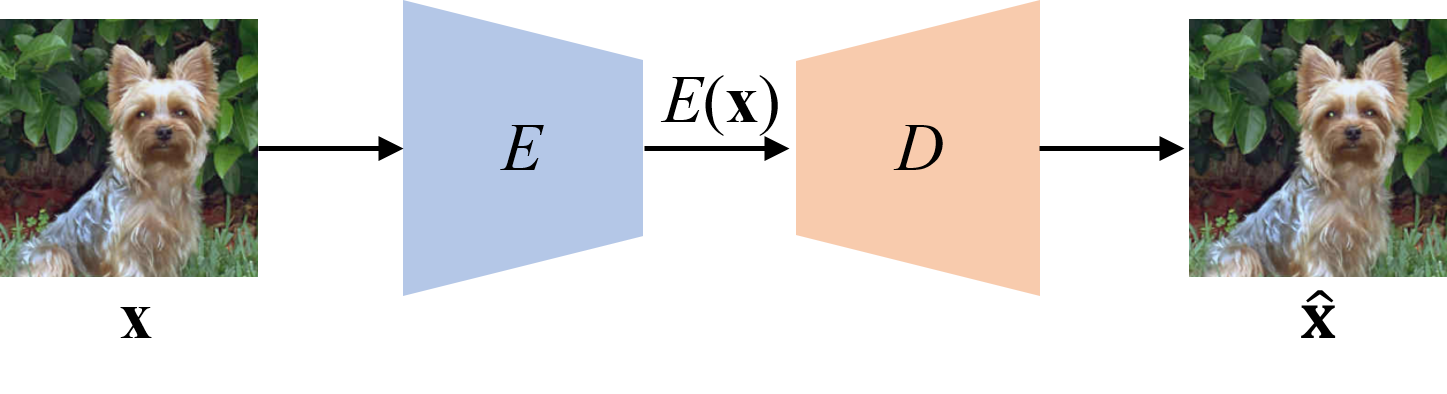
\includegraphics[width=\textwidth]{Figures/AED.png}
        \caption{AutoEncoding Data (AED)}
    \end{subfigure}\\\vspace{2mm}
    ~ %add desired spacing between images, e. g. ~, \quad, \qquad, \hfill etc.
      %(or a blank line to force the subfigure onto a new line)
    \begin{subfigure}[c]{0.33\textwidth}
        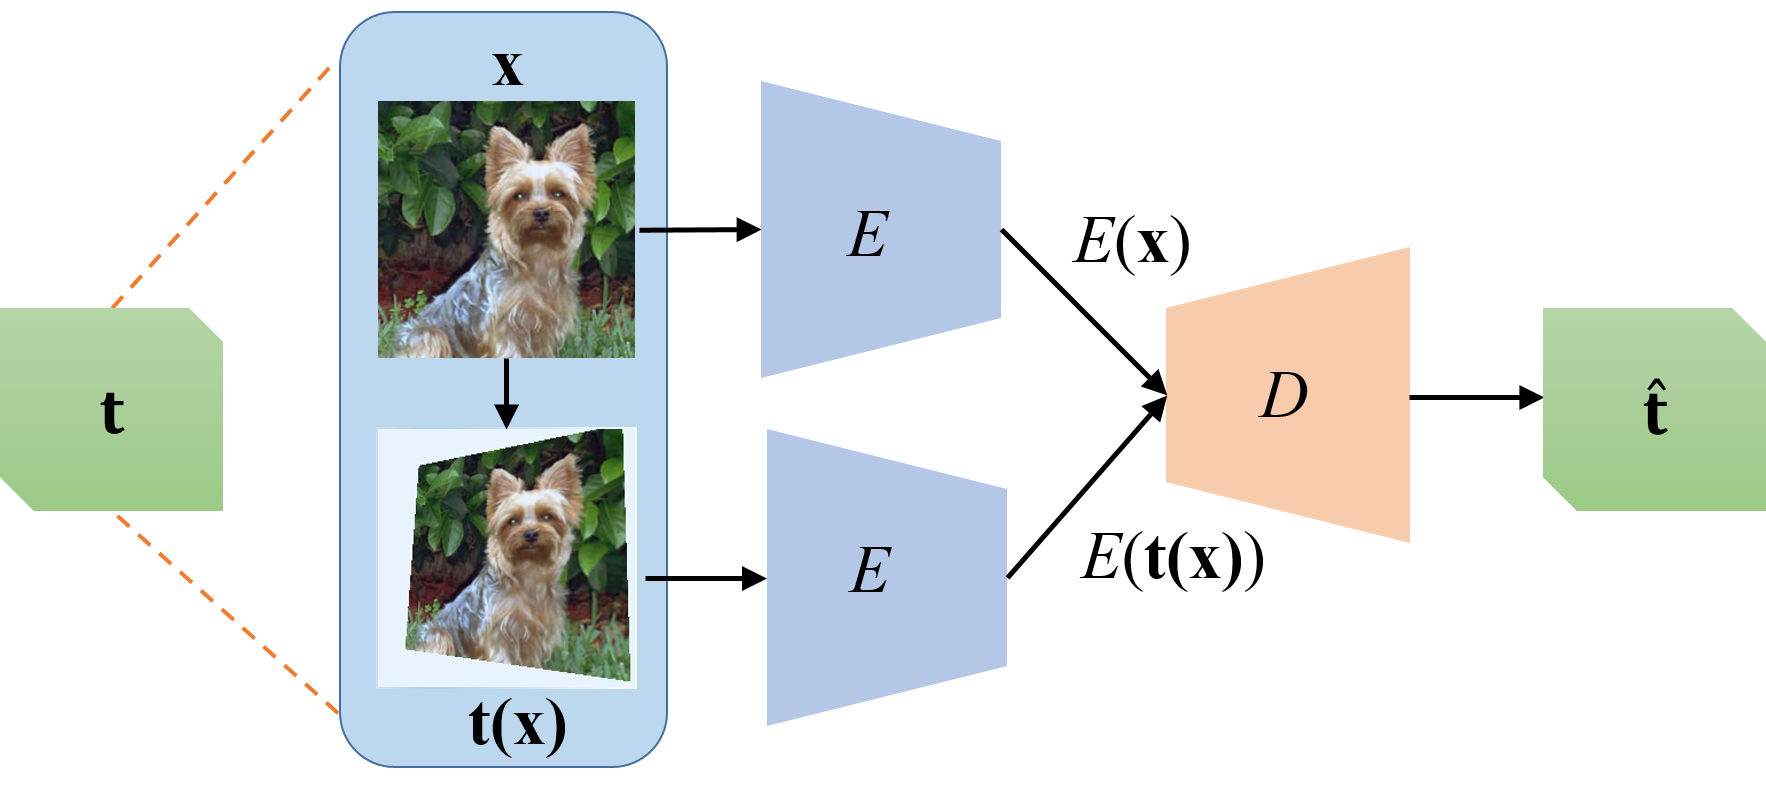
\includegraphics[width=\textwidth]{Figures/AET.png}
        \caption{AutoEncoding Transformation (AET)}
    \end{subfigure}\\\vspace{2mm}
    \begin{subfigure}[c]{0.33\textwidth}
        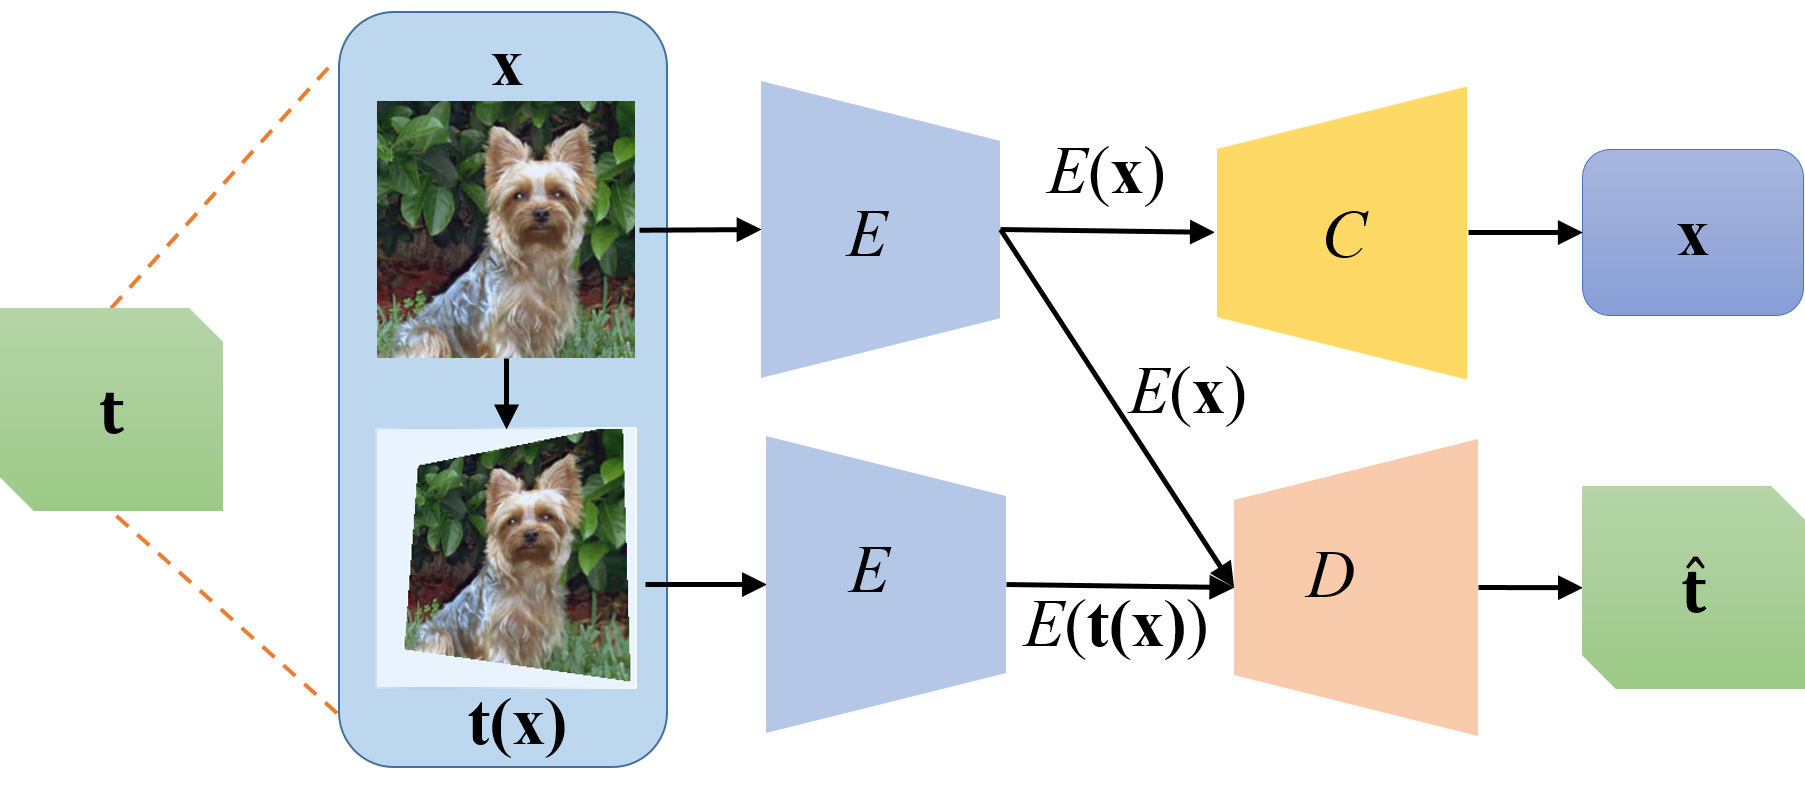
\includegraphics[width=\textwidth]{Figures/SAT.png}
        \caption{(Semi-)Supervised Autoencoding Transformation (SAT)}
    \end{subfigure}
    \caption{The figure illustrates a comparison between AED, AET, and AET. The AED and AET seek to reconstruct the input data and transformation at the output end, respectively. The encoder (E) extracts the representation of input and transformed images. The decoder (D) either reconstructs the data in AED, or the transformation in AET. The SAT builds a classifier (C) upon the output representation from the encoder by capturing the equivariant visual structures under various transformations. }\label{fig:comparison}
    %\vspace{-5mm}
\end{figure}


% The very first letter is a 2 line initial drop letter followed
% by the rest of the first word in caps (small caps for compsoc).
%
% form to use if the first word consists of a single letter:
% \IEEEPARstart{A}{demo} file is ....
%
% form to use if you need the single drop letter followed by
% normal text (unknown if ever used by the IEEE):
% \IEEEPARstart{A}{}demo file is ....
%
% Some journals put the first two words in caps:
% \IEEEPARstart{T}{his demo} file is ....
%
% Here we have the typical use of a "T" for an initial drop letter
% and "HIS" in caps to complete the first word.

\IEEEPARstart{I}n this paper, we aspire to show that {\em transformations} play a fundamental role in learning powerful representations by transforming images as a means to reveal the intrinsic patterns from transformed visual structures. Particularly,
Transformation Equivariant Representation (TER) learning seeks to model representations that equivary to various transformations on images.
In other words, the representation of an image ought to change in the same way as it is transformed. This is motivated by the assumption that image representations should capture the intrinsic visual structures such that transformations can be decoded from the representations of original and transformed images. Based on this assumption, we formally present a novel criterion of AutoEncoding Transformations (AET) to learn the TERs for various groups of transformations.


Learning the TERs has been adopted in Hiton's seminal work on learning transformation equivariant capsules \cite{hinton2011transforming}, and plays a critical role for the success of Convolutional Neural Networks (CNNs) \cite{krizhevsky2012imagenet}. Specifically, the representations learned by the CNNs are translation equivariant as their feature maps are shifted in the same way as input images are translated. On top of these feature maps that preserve the visual structures of translation equivariance, fully connected layers are built to output the predicted labels of input images.

Obviously, the translation equivariant convolutional features play the pivotal role in delivering the state-of-the-art performances in the deep networks. Thus, they are extended beyond translations to learn more expressive representations of equivariance to generic types of transformations, such as affine, projective and homographic transformations. Aline this direction, the group equivariant CNNs \cite{cohen2016group}
are developed to guarantee the transformation of input images results in the same transformation of input images.


However, the group equivariant CNNs \cite{cohen2016group} and their variants \cite{cohen2016steerable,lenssen2018group} are restricted to discrete transformations, and the resultant representations are also limited to a group representation of linear transformations. These limitations restrict their abilities to model group representations of complex transformations that could be continuous and nonlinear in many learning tasks, ranging from unsupervised, to semi-supervised and supervised learning.



\subsection{Unsupervised Learning of Transformation Equivariant Representations}

The focus of this paper is on the principle of autoencoding transformations and its application to learn the transformation equivariant representations. The core idea is to encode data with the representations from which the transformations can be decoded as much as possible. We will begin with an unsupervised learning of such representations without involving any labeled data, and then proceed to a generalization to semi-supervised and supervised representations by encoding label information as well.

Unlike group equivariant CNNs that learn the feature maps mathematically satisfying the transformation equivariance as a function of the group of transformations, the proposed AutoEncoding Transformations (AET) presents an autoencoding architecture to learn transformation equivariant representations by reconstructing applied transformations. As long as a transformation of input images results in equivariant representations, it should be well decoded from the representations of original and transformed images.  Compared with the group equivariant CNNS, the AET model is more flexible and tractable to tackle with any transformations and their compositions, since it does not rely on a strict convolutional structure to

The AET is also in contrast to the conventional AutoEncoding Data (AED) paradigm that instead aims to reconstruct data rather than the transformations. Figure \ref{fig:comparison}(a) and (b) illustrate the comparison between the AET and AED. Since the space of transformations (e.g., the few parameters of transformations) is of quite lower dimension than that of data space (e.g., the pixel space of images), the decoder of the AET can be quite shallower than that of the AED. This allows the backpropagated errors to more sufficiently train the encoder that models the representations of input data in the AET architecture.

Moreover, an AET model can be trained from an information-theoretic perspective by maximizing the information in the learned representation about the applied transformation and the input data. This will generalize the group representations of linear transformations to more general forms that could equivary nonlinearly to input transformations. It results in Generalized Transformation Equivariant Representations (GTERs) that can capture more complex patterns of visual structure under transformations. Unfortunately, this will result in an intractable optimization problem to maximize the mutual information between representations and transformations. A variational lower bound of the mutual information can be derive by introducing a surrogate transformation decoder, yielding a novel model of Autoencoding Variational Transformation (AVT) as an alterative to the deterministic AET.






\subsection{(Semi-)Supervised Learning of Transformation Equivariant Representations}


While both AET and AVT are trained in an unsupervised fashion, they can act as the basic representation for building the (semi-)supervised classifiers. Along this direction, we can train (Semi-)Supervised Autoencoding Transformation (SAT) that jointly trains the transformation equivariant representations as well as the corresponding classifiers.

Figure \ref{fig:comparison}(c) illustrates the SAT model, where a classifier head is added upon the representation encoder of an AET network.  The SAT can be based on either the deterministic AET or the probabilistic AVT architecture. Particularly, along the direction pointed by the AVT, we seek to train the proposed (semi-)supervised transformation equivariant classifiers by maximizing the mutual information of the learned representations with the transformations and labels. In this way, the trained SAT model can not only handle the transformed data through their equivarying representations, but also encode the labeling information through the supervised classifier. The resultant SAT also contains the deterministic model based on the AET as a special case by fixing a deterministic model to representation encoder and the transformation decoder.

The transformation equivariance in the SAT model is contrary to the data augmentation by transformations in deep learning literature \cite{krizhevsky2012imagenet}. First, the data augmentation is only applicable to augment the labeled examples for model training, which cannot be extended to unlabeled data. This limits it in semi-supervised learning by exploring the unlabeled data. Second, the data augmentation aims to enforce the transformation invariance, in which the labels of transformed data are supposed to be invariant. This differs from the motivation to encode the inherent visual structures that equivary under various transformations.


Actually, in the (semi-)supervised transformation equivariant classifiers, we aim to integrate the principles of both training {\em transformation equivariant representations} and {\em transformation invariant classifiers} seamlessly. Indeed, both principles have played the key role in compelling performances of the CNNs and their modern variants. This is witnessed by the translation equivariant convolutional feature maps and the atop classifiers that are supposed to make transformation-invariant predictions with the spatial pooling and fully connected layers. We will show that the proposed SAT extends the translation equivariance in the CNNs to cover a generic class of transformation equivariance, as well as encode the labels to train the representations and the associated transformation invariant classifiers. We hope this can deepen our understanding of the interplay between the transformation equivariance and invariance both of which play the fundamental roles in training robust classifiers with labeled and unlabeled data.

The remainder of this paper is organized as follows. We will review the related works in Section~\ref{sec:related}.  The unsupervised and (semi-)supervised learning of transformation equivariant representations will be presented in the autoencoding transformation framework in Section~\ref{sec:unsup} and Section~\ref{sec:sup}, respectively.  We will present experiment results in Section~\ref{sec:unexp} and Section~\ref{sec:supexp} for unsupervised and semi-supervised tasks. We will conclude the paper and discuss the future works in Section~\ref{sec:concl}.

\section{Related Works}\label{sec:related}
In this section, we will review the related works on learning transformation-equivariant representation, as well as unsupervised and (semi-)supervised models.

\subsection{Transformation-Equivariant Representations}
Learning transformation-equivariant representations can trace back to the seminal work on training capsule nets \cite{sabour2017dynamic,hinton2011transforming,hinton2018matrix}. The transformation equivariance is characterized by the various directions of capsules, while the confidence of belonging to a particular class is captured by their lengths.
%However, there was a lack of explicit training mechanism to ensure the resultant capsules be of transformation equivariance.

Many efforts have been made in literature  \cite{cohen2016group,cohen2016steerable,lenssen2018group} on extending the conventional translation-equivariant convolutions to cover more transformations.
Among them are group equivariant convolutions (G-convolution) \cite{cohen2016group} that have been developed to equivary to more types of transformations. The idea of group equivariance has also been introduced to the capsule nets \cite{lenssen2018group} by ensuring the equivariance of output pose vectors to a group of transformations with a generic routing mechanism. However, the group equivariant convolution is restricted to discrete transformations, which limits its ability to learn the representations equivariant to generic continuous transformations.


%However, these group equivariant convolutions and capsules must be trained in a supervised fashion \cite{cohen2016group,lenssen2018group} with labeled data for specific tasks, instead of learning unsupervised transformation-equivariant representations generalizable to unseen tasks. Moreover, their representations are restricted to be a function of groups, which limits the ability of training future classifiers on top of more flexible representations.


%Recently, Zhang et al.~\cite{zhang2019aet} present a novel Auto-Encoding Transformation (AET) model by learning a representation from which an input transformation can be reconstructed. This is closely related to our motivation of learning transformation equivariant representations, considering the transformation can be decoded from the learned representation of original and transformed images. On the contrary, in this paper, we approach it from an information-theoretic point of view in a more principled fashion.
%
%
%Specifically, we will define a joint probability over the representations and transformations, and this will enable us to train unsupervised representations by directly maximizing the mutual information between the transformations and the representations. We wish the resultant representations can generalize to new tasks without access to their labels beforehand.


\subsection{Unsupervised Representation Learning}
{\noindent \bf Auto-Encoders and GANs.}
Unsupervised auto-encoders have been extensively studied in literature \cite{hinton1994autoencoders,japkowicz2000nonlinear,vincent2008extracting}. Existing auto-encoders are trained by reconstructing input {\em data} from the outputs of encoders.
%The encoders seek to extract features to compactly represent the most essential information about input data so that the paired decoders can recover the input data from the extracted features.
A large category of auto-encoder variants have been proposed.
Among them is the Variational Auto-Encoder (VAE) \cite{kingma2013auto} that maximizes the lower-bound of the data likelihood to train a pair of probabilistic encoder and decoder, while beta-VAE seeks to disentangle representations by introducing an adjustable hyperparameter on the capacity of latent channel to balance between the independence constraint and the reconstruction accuracy \cite{higgins2017beta}.  Denoising auto-encoders \cite{vincent2008extracting}
attempt to reconstruct noise-corrupted data to
learn robust representations, while
contrastive Auto-Encoders \cite{rifai2011contractive} encourage to learn representations invariant to small perturbations on data.
%Zhang et al.~\cite{zhang2017split} present a cross-channel auto-encoder by reconstructing a subset of data channels from another subset with the cross-channel features being concatenated as data representation.
Along this direction, Hinton et al.~\cite{hinton2011transforming} propose capsule networks to explore transformation equivariance by minimizing the discrepancy between the reconstructed and target data.

On the other hand, Generative Adversarial Nets (GANs) have also been used to train unsupervised representations.  Unlike the auto-encoders, the GANs \cite{goodfellow2014generative} and their variants \cite{donahue2016adversarial,dumoulin2016adversarially,qi2017loss,arjovsky2017wasserstein} generate data from the noises drawn from a simple distribution, with a discriminator trained adversarially to distinguish between real and fake data. The sampled noises can be viewed as the representation of generated data over a manifold, and one can train an encoder by inverting the generator to find the generating noise. This can be implemented by jointly training a pair of mutually inverse generator and encoder \cite{donahue2016adversarial,dumoulin2016adversarially}. There also exist better generalizable GANs in producing unseen data based on the Lipschitz assumption on the real data distribution \cite{qi2017loss,arjovsky2017wasserstein}, which can give rise to more powerful representations of data out of training examples  \cite{donahue2016adversarial,dumoulin2016adversarially,edraki2018generalized}. Compared with the Auto-Encoders, GANs do not rely on learning one-to-one reconstruction of data; instead, they aim to generate the entire distribution of data.




{\noindent \bf Self-Supervisory Signals.} There exist many other unsupervised learning methods using different types of self-supervised signals to train deep networks.
%These self-supervised signals can be directly derived from data themselves without having to be manually labeled.
Mehdi and Favaro~\cite{noroozi2016unsupervised} propose to solve Jigsaw puzzles to train a convolutional neural network.
Doersch et al.~\cite{doersch2015unsupervised} train the network by inferring the relative positions between sampled patches from an image as self-supervised information. Instead, Noroozi et al.~\cite{noroozi2017representation} count features that satisfy equivalence relations between downsampled and tiled images. Gidaris et al.~\cite{gidaris2018unsupervised} propose to train RotNets by predicting a discrete set of image rotations, but they are unable to handle generic continuous transformations and their compositions. Dosovitskiy et al.~\cite{dosovitskiy2014discriminative} create a set of surrogate classes by applying various transformations to individual images. However, the resultant features could over-discriminate visually similar images as they always belong to different surrogate classes.
Unsupervised features have also been learned from videos by estimating the self-motion of moving objects between consecutive frames \cite{agrawal2015learning}.

\subsection{(Semi-)Supervised Representation Learning}

In addition, there exist a large number of semi-supervised models in literature. Here, we particularly mention three  state-of-the-art methods that will be compared in experiments.  Temporal ensembling \cite{laine2016temporal} and mean teachers \cite{tarvainen2017mean} both use an ensemble of teachers to supervise the training of a student model. Temporal ensembling uses the exponential moving average of predictions made by past models on unlabeled data as targets to train the student model. Instead, mean teachers update the student model with the exponential moving average of the weights of past models. On the contrary, the Virtual Adversarial Training (VAT) \cite{miyato2018virtual} seeks to minimizes the change of predictions on unlabeled examples when their output values are adversarially altered. This could result in a robust model that prefers smooth predictions over unlabeled data.


The SAT also differs from transformation-based data augmentation in which the transformed samples and their labels are used directly as additional training examples \cite{krizhevsky2012imagenet}. First, in the semi-supervised learning, unlabeled examples cannot be directly augmented to form training examples due to their missing labels. Moreover, data augmentation needs to preserve the labels on augmented images, and this prevents us from applying the transformations that could severely distort the images (e.g., shearing, rotations with arbitrary angles, and projective transformations) or invalidate the associated labels (e.g., vertically flipping ``6" to ``9").
%Even small perturbations (transformations) can create adversarial examples with the invalidate labels training examples to attack the model training.
In contrast, the SAT avoids using the labels of transformed images to supervisedly train the classifier directly; instead it attempts to encode the visual structures of images equivariant to various transformations without access to their labels. This leads to a label-blind TER regularizer to explore the unlabeled examples for the semi-supervised problem.

\section{Unsupervised Learning of Transformation Equivariant Representations}\label{sec:unsup}

In this section, we will first present the autoencoding transformation architecture to learn the transformation equivariant representations in a deterministic fashion. Then, a variational alternative approach will be presented to handle the uncertainty in the representation learning by maximizing the mutual information between the learned representations and the applied transformations.


\subsection{AET: A Deterministic Model}

We begin by defining the notations used in the proposed AutoEncoding Transformation (AET) architecture.
Consider a random transformation $\mathbf t$ sampled from a transformation distribution $p(\mathbf t)$ (e.g., warping, projective and homographic transformations), as well as an image $\mathbf x$ drawn from a data distribution $p(\mathbf x)$ in a sample space $\mathcal X$. Then the application of $\mathbf t$ to $\mathbf x$ results in a transformed image $\mathbf t(\mathbf x)$.

The goal of AET focuses on learning a representation encoder $E_\theta: \mathbf x \mapsto E_\theta(\mathbf x)$ with parameters $\theta$, which maps a sample $\mathbf x\sim p(\mathbf x)$ to its representation $E_\theta(\mathbf x)$ in a linear space $\mathcal Z$.
For this purpose, one need to learn a transformation decoder with parameters $\phi$
$$
D_\phi: \left[E_\theta(\mathbf x), E_\theta(\mathbf t(\mathbf x))\right]\mapsto \hat {\mathbf t}
$$
that makes an estimate $\hat{\mathbf t}$ of the input transformation $\mathbf t$ from the representations of original and transformed samples. Since the transformation decoder takes the encoder outputs rather than original and transformed images, this pushes the encoder to capture the inherent visual structures of images to make a satisfactory estimate of the transformation.

Then the AET can be trained to jointly learn the representation encoder $E_\theta$ and the transformation decoder $D_\phi$. A loss function $\ell(\mathbf t, \hat{\mathbf t})$ measuring the deviation between a transformation $\mathbf t$ and its estimate $\hat{\mathbf t}$ is minimized to train the AET over $p(\mathbf t)$ and $p(\mathbf x)$:
\begin{equation}\label{eq:AET_loss}
\min_{\theta,\phi} \mathop\mathbb E\limits_{\mathbf t \sim p(\mathbf t), \mathbf x\sim p(\mathbf x)}\ell(\mathbf t, \hat{\mathbf t})
\end{equation}
where the estimated transformation $\hat{\mathbf t}$ can be written as a function of the encoder $E_\theta$ and the decoder $D_\phi$ such that
$$
\hat{\mathbf t}= D_\phi\left[E_\theta(\mathbf x), E_\theta(\mathbf t(\mathbf x))\right],
$$
and the expectation $\mathbb E$ is taken over the distributions of transformations and data.
%Like in training other deep neural networks,

In this way, the encoder $E_\theta$ and the decoder $D_\phi$ can be jointly trained over mini-batches by back-propagating the gradient of the loss $\ell$ to update their parameters.

\subsection{AVT: A Probabilistic Model}

Alternatively, we can train transformation equivariant representations to contain as much information as possible about applied transformations to recover them.


\begin{figure*}[t]
%\captionsetup[subfigure]{singlelinecheck=false}
    \centering
    \begin{subfigure}[c]{0.49\textwidth}
        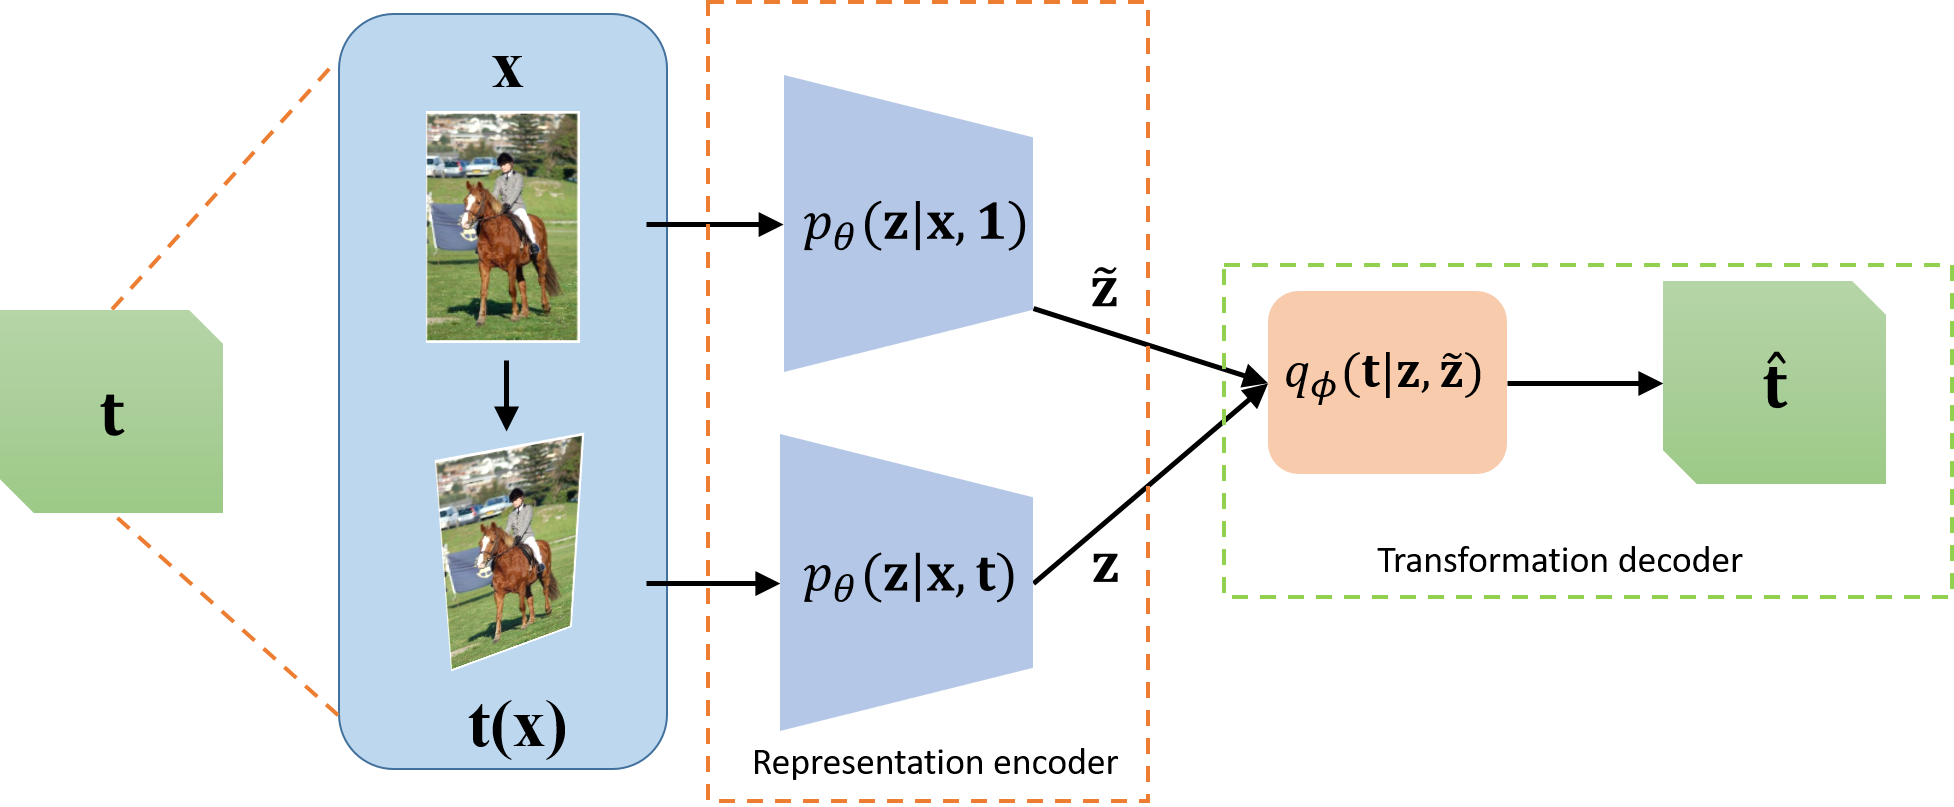
\includegraphics[width=\textwidth]{Figures/AVT.png}
        \caption{Autoencoding Variational Transformations (AVT)}
    \end{subfigure}
    ~ %add desired spacing between images, e. g. ~, \quad, \qquad, \hfill etc.
      %(or a blank line to force the subfigure onto a new line)
    \begin{subfigure}[c]{0.49\textwidth}
        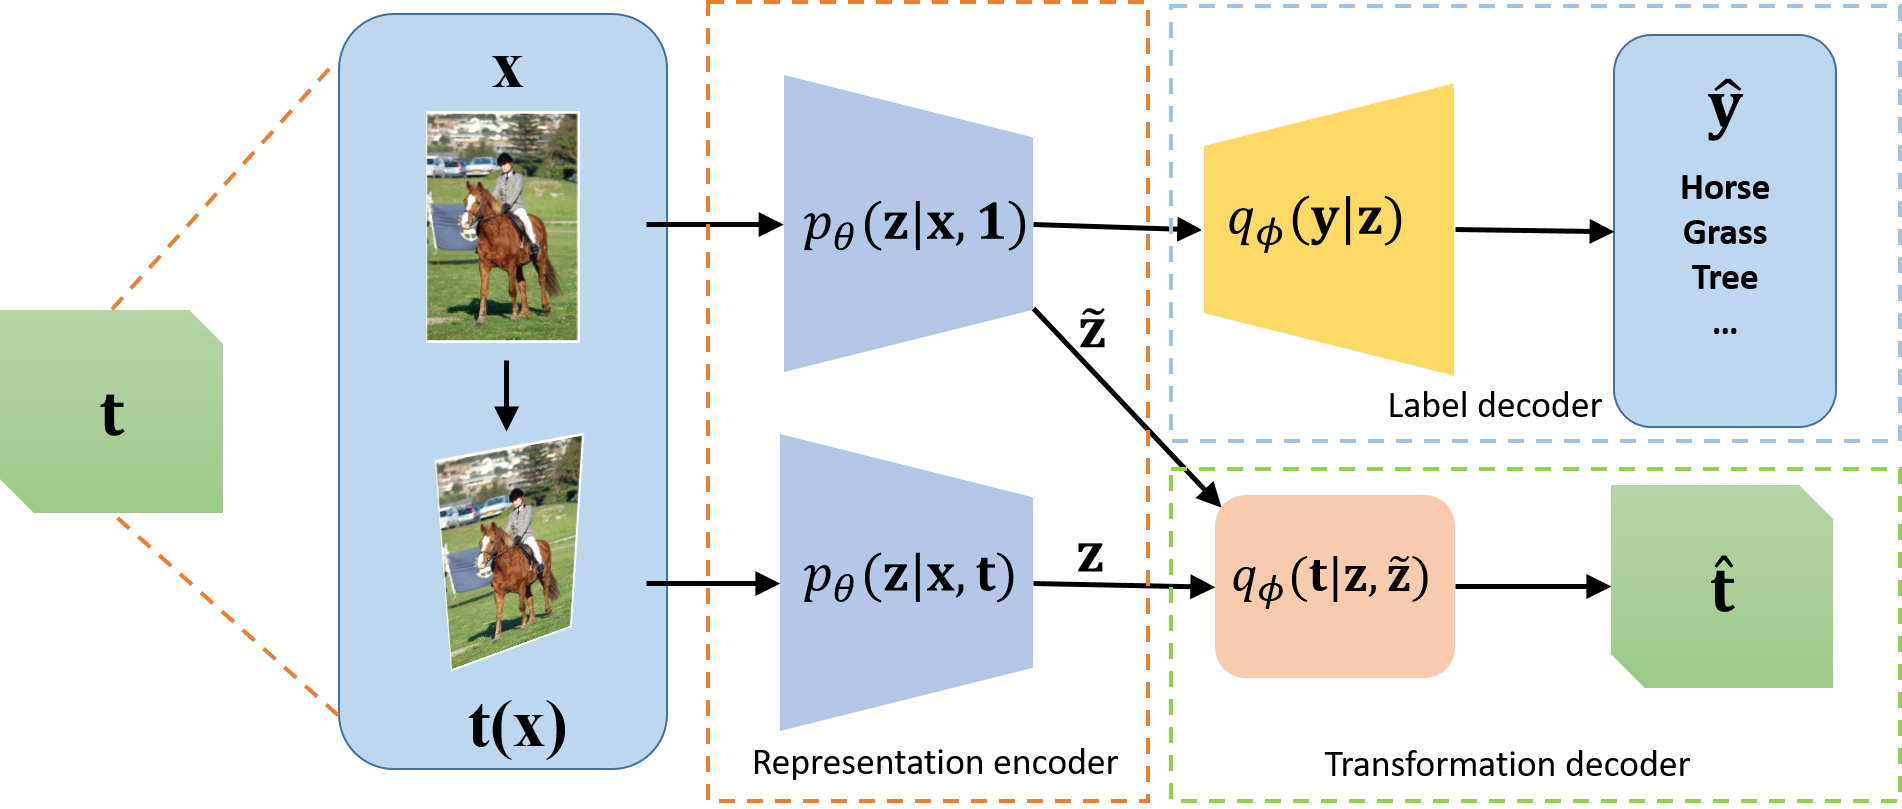
\includegraphics[width=\textwidth]{Figures/vSAT.png}
        \caption{(Semi-)Supervised Autoencoding Transformations (SAT)}
    \end{subfigure}\\
    \caption{The figure illustrates the variational approach to unsupervised learning and (semi-)supervised learning of autoencoding transformations, namely AVT and SAT respectively. The probability $p_\theta(\mathbf z|\mathbf t,\mathbf x)$ acts as the representation encoder, while $q_\phi(\mathbf t|\mathbf z,\mathbf {\tilde z})$ and $q_\phi(\mathbf y|\mathbf {\tilde z})$ play the roles of a transformation and label decoder, respectively. By setting the transformation to an identity $\mathbf 1$, the corresponding $\tilde{\mathbf z}$ is the representation of an original image.}\label{fig:variational}
    %\vspace{-5mm}
\end{figure*}

\subsubsection{Notations}
Formally, our goal is to learn an encoder that maps a transformed sample $\mathbf t(\mathbf x)$ to a probabilistic representation with the mean $f_\theta$ and variance $\sigma_\theta$. This results in the following probabilistic representation $\mathbf z \in \mathcal Z$ of $\mathbf t(\mathbf x)$:
\begin{equation}\label{eq:rep_t}
\mathbf z = f_\theta(\mathbf t(\mathbf x))+\sigma_\theta(\mathbf t(\mathbf x)) \circ \epsilon
\end{equation}
where $\epsilon$ is sampled from a normal distribution $p(\epsilon)\triangleq\mathcal N(\epsilon|\mathbf 0, \mathbf I)$ with $\circ$ denoting the element-wise product. Thus, the resultant probabilistic representation $\mathbf z$ follows a normal distribution
$$
p_\theta(\mathbf z|\mathbf t, \mathbf x)\triangleq \mathcal N\left(\mathbf z|f_\theta(\mathbf t(\mathbf x)),\sigma_\theta^2(\mathbf t(\mathbf x))\right)
$$
conditioned on the randomly sampled transformation $\mathbf t$ and input data $\mathbf x$.

On the other hand, the representation of the original sample $\mathbf x$ is a special case when $\mathbf t$ is an identity transformation, which is
\begin{equation}\label{eq:rep_ori}
\mathbf {\tilde z} = f_\theta(\mathbf x)+\sigma_\theta(\mathbf x) \circ \tilde \epsilon
\end{equation}
whose mean and variance are computed by using the deep network with the same weights $\theta$, and $\tilde \epsilon \sim p(\tilde\epsilon)\triangleq\mathcal N(\tilde\epsilon|\mathbf 0, \mathbf I)$.

\subsubsection{Generalized Transformation Equivariance}
In the conventional definition of transformation equivariance, there should exist an automorphism $\boldsymbol\rho(\mathbf t)\in {\rm Aut}(\mathcal Z):\mathcal Z \rightarrow \mathcal Z$ in the representation space, such that \footnote{The transformation $\mathbf t$ in the sample space $\mathcal X$ and the corresponding transformation $\boldsymbol\rho$ in the representation space $\mathcal Z$ need not be the same. But the representation transformation $\boldsymbol\rho(\mathbf t)$ should be a function of the sample transformation $\mathbf t$. }
$$
\mathbf z = [\boldsymbol\rho (\mathbf t)](\mathbf {\tilde z})
$$
Here the transformation $\boldsymbol\rho(\mathbf t)$ is independent of the input sample $\mathbf x$. In other words, the representation $\mathbf z$ of a transformed sample is completely determined by the original representation $\mathbf {\tilde z}$ and the applied transformation $\mathbf t$ with no need to access the sample $\mathbf x$. This is called {\em steerability} property in literature \cite{cohen2016steerable}, which enables us to compute  $\mathbf z$ by applying the sample-independent transformation directly to the original representation $\mathbf {\tilde z}$.

This property can be generalized without relying on the linear group representations of transformations through automorphisms. Instead of sticking with a linear $\boldsymbol\rho(\mathbf t)$, one can seek a more general relation between $\mathbf z$ and $\mathbf {\tilde z}$, independently of $\mathbf x$.  From an information theoretical point of view, this requires $(\mathbf {\tilde z},\mathbf t)$ should jointly contain all necessary information about $\mathbf z$ so that $\mathbf z$ can be best estimated from them without a direct access to $\mathbf x$.

%this can be done by maximizing the dependence between $\mathbf z$ and $\{\mathbf {\tilde z},\mathbf t\}$, so that $\mathbf z$ can be best estimated from $\mathbf {\tilde z}$ and $\mathbf t$.

This leads us to maximizing the mutual information $I_\theta(\mathbf z;\mathbf {\tilde z},\mathbf t)$ to learn the generalized transformation equivariant representations. Indeed, by the chain rule and the nonnegativity of mutual information, we have
$$
I_\theta(\mathbf z;\mathbf {\tilde z},\mathbf t)= I_\theta(\mathbf z;\mathbf {\tilde z},\mathbf t, \mathbf x) - I_\theta(\mathbf z;\mathbf x|\mathbf {\tilde z},\mathbf t) \leq I_\theta(\mathbf z;\mathbf {\tilde z},\mathbf t, \mathbf x),
$$
which shows $I_\theta(\mathbf z;\mathbf {\tilde z},\mathbf t)$ is upper bounded by the mutual information $I_\theta(\mathbf z;\mathbf {\tilde z},\mathbf t, \mathbf x)$ between $\mathbf z$ and $(\mathbf {\tilde z},\mathbf t,\mathbf x)$.

Clearly, when $I_\theta(\mathbf z;\mathbf x|\mathbf {\tilde z},\mathbf t)=0$, $I_\theta(\mathbf z;\mathbf {\tilde z},\mathbf t)$ attains the maximum value of its upper bound $I_\theta(\mathbf z;\mathbf {\tilde z},\mathbf t, \mathbf x)$. In this case, $\mathbf x$ would provide no more information about $\mathbf z$ than $(\mathbf {\tilde z},\mathbf t)$, which implies one can estimate $\mathbf z$ directly from $(\mathbf {\tilde z},\mathbf t)$ without accessing $\mathbf x$.
Thus, we propose to solve
%The left hand side is the mutual information about $\mathbf z$ from the joint $\{\mathbf {\tilde z},\mathbf t\}$ and $\mathbf x$. This equality suggests that the maximum value of $I_\theta(\mathbf z;\mathbf {\tilde z},\mathbf t)$ attains when $I_\theta(\mathbf z;\mathbf x|\mathbf {\tilde z},\mathbf t)=0$, implying  that $\mathbf x$ provides no additional information about $\mathbf z$ given $\{\mathbf {\tilde z},\mathbf t\}$, and one can estimate $\mathbf z$ directly from its dependence on $\{\mathbf {\tilde z},\mathbf t\}$.
%Thus, we propose to maximize
$$
\theta^\star = \arg\max_{\theta} I_\theta(\mathbf z;\mathbf {\tilde z},\mathbf t)
$$
to learn the probabilistic encoder $\theta^\star$ in pursuit of such a generalized TER.

%We can decompose it into two components
%$$
%I_\theta(\mathbf z;\mathbf {\tilde z},\mathbf t)=I_\theta(\mathbf z;\mathbf {\tilde z})+I_\theta(\mathbf z;\mathbf t|\mathbf {\tilde z})
%$$
%The first term accounts for the transformation-invariant component that reveals the information in the representation of the transformed sample about the original representation. Ideally, this component could be maximized if there is a transformation-invariant bijection between the representations before and after the transformation.
%
%The second term is the transformation-equivariant component. It reveals the information about the applied transformation $\mathbf t$ in the representation $\mathbf z$ of a transformed sample, when the original representation is given.

%maximize the dependence between $\mathbf z$ and $\mathbf {\tilde z}$ can be calculated from $\mathbf {\tilde z}$ and the applied transformation $\mathbf t$.

%\subsubsection{Formulation}


%Then, a joint distribution
%\begin{equation}\label{eq:joint}
%p_\theta(\mathbf z,\mathbf t|\mathbf x)=p(\mathbf t)p_\theta(\mathbf z|\mathbf t,\mathbf x)
%\end{equation}
%between the transformation $\mathbf t$ and the representation $\mathbf z$ can be defined, and the mutual information $I_\theta(\mathbf t,\mathbf z|\mathbf x)$ between $\mathbf z$ and $\mathbf t$ follows as a function of the joint distribution to characterize the transformation equivariance from an information-theoretic perspective -- the larger the mutual information, the more information about $\mathbf t$ can be inferred from the representation $\mathbf z$.
%
%Therefore, a transformation equivariant representation $\mathbf z$ can be learned by maximizing
% the expected mutual information over the data distribution $p(\mathbf x)$
%$$
%\max_{\theta} \mathop \mathbb E\limits_{\mathbf x\sim p(\mathbf x)} I_\theta(\mathbf t,\mathbf z|\mathbf x)
%$$

However, a direction maximization of the above mutual information needs to evaluate an intractable posterior $p_\theta(\mathbf t|\mathbf z,\mathbf {\tilde z})$ of the transformation. Thus, we instead lower bound the mutual information by introducing a surrogate decoder $q_\phi(\mathbf t|\mathbf z,\mathbf {\tilde z})$ with the parameters $\phi$ to approximate the true posterior.

\subsubsection{Variational Approach}

Unlike the variational autoencoder that lower-bounds data likelihood \cite{kingma2013auto}, we directly take a lower bound of the mutual information \cite{agakov2004algorithm} between  $\mathbf z$ and $(\mathbf {\tilde z},\mathbf t)$ below
%\[
%\begin{aligned}
%&I_\theta(\mathbf t,\mathbf z|\mathbf x) = H(\mathbf t|\mathbf x) - H(\mathbf t|\mathbf z,\mathbf x)\\
%&=H(\mathbf t|\mathbf x) +\mathop\mathbb E\limits_{p_\theta(\mathbf t,\mathbf z|\mathbf x)} \log p_\theta(\mathbf t|\mathbf z,\mathbf x)\\
%&= H(\mathbf t|\mathbf x)  + \mathop\mathbb E\limits_{p_\theta(\mathbf t,\mathbf z|\mathbf x)} \log q_\phi(\mathbf t|\mathbf z,\mathbf x)\\
%&+ D(p_\theta(\mathbf t,\mathbf z|\mathbf x)\|q_\phi(\mathbf t,\mathbf z|\mathbf x))\\
%&\geq H(\mathbf t|\mathbf x)  + \mathop\mathbb E\limits_{p_\theta(\mathbf t,\mathbf z|\mathbf x)} \log q_\phi(\mathbf t|\mathbf z,\mathbf x) \triangleq \tilde I_{\theta,\phi}(\mathbf t,\mathbf z|\mathbf x)
%\end{aligned}
%\]
\[
\begin{aligned}
&I_\theta(\mathbf z; \mathbf {\tilde z},\mathbf t) = I_\theta(\mathbf z; \mathbf {\tilde z}) + I_\theta(\mathbf z; \mathbf t|\mathbf {\tilde z})\\
&\geq I_\theta(\mathbf z; \mathbf t|\mathbf {\tilde z})
= H(\mathbf t|\mathbf {\tilde z}) - H(\mathbf t|\mathbf z,\mathbf {\tilde z})\\
&=H(\mathbf t|\mathbf {\tilde z}) +\mathop\mathbb E\limits_{p_\theta(\mathbf t,\mathbf z,\mathbf {\tilde z})} \log p_\theta(\mathbf t|\mathbf z,\mathbf {\tilde z})\\
&= H(\mathbf t|\mathbf {\tilde z})  + \mathop\mathbb E\limits_{p_\theta(\mathbf t,\mathbf z,\mathbf {\tilde z})} \log q_\phi(\mathbf t|\mathbf z,\mathbf {\tilde z})\\
&+ \mathop\mathbb E\limits_{p(\mathbf z,\mathbf {\tilde z})} D(p_\theta(\mathbf t|\mathbf z,\mathbf {\tilde z})\|q_\phi(\mathbf t|\mathbf z,\mathbf {\tilde z}))\\
&\geq H(\mathbf t|\mathbf {\tilde z})  + \mathop\mathbb E\limits_{p_\theta(\mathbf t,\mathbf z,\mathbf {\tilde z})} \log q_\phi(\mathbf t|\mathbf z,\mathbf {\tilde z}) \triangleq \tilde I_{\theta,\phi}(\mathbf z;\mathbf {\tilde z},\mathbf t)
\end{aligned}
\]
where $H(\cdot)$ denotes the (conditional) entropy, and $D(p_\theta(\mathbf t|\mathbf z,\mathbf {\tilde z})\|q_\phi(\mathbf t|\mathbf z,\mathbf {\tilde z}))$ is the non-negative Kullback divergence between $p_\theta$ and $q_\phi$.

We choose to maximize the lower variational bound $\tilde I_{\theta,\phi}(\mathbf z;\mathbf {\tilde z},\mathbf t)$. Since $H(\mathbf t|\mathbf {\tilde z})$ is nonnegative and independent of the model parameters $\theta$ and $\phi$, we choose to solve
\begin{equation}\label{eq:var}
\begin{aligned}
&\max\limits_{\theta,\phi}~\mathcal L^{\rm unsup}_{\theta,\phi} \triangleq \mathop\mathbb E\limits_{p_\theta(\mathbf t,\mathbf z,\mathbf {\tilde z})}\log q_\phi(\mathbf t|\mathbf z,\mathbf {\tilde z})\\
&=\mathop\mathbb E\limits_{p(\mathbf x),p(\mathbf t)} \mathop\mathbb E\limits_{p(\epsilon),p(\tilde\epsilon)}\log q_\phi(\mathbf z,\mathbf {\tilde z})\\
\end{aligned}
\end{equation}
to learn $\theta$ and $\phi$ under the expectation over $p(\mathbf t, \mathbf z, \mathbf {\tilde z})$, and the equality follows from the generative process for the representations in Eqs.~(\ref{eq:rep_t})--(\ref{eq:rep_ori}).

%This variational approach differs from the variational auto-encoders \cite{kingma2013auto}: the latter attempts to lower bound the data loglikelihood, while we instead seek to lower bound the mutual information here. Although both are derived based on an auto-encoder structure, the mutual information has a simpler form of lower bound than the data likelihood -- it does not contain an additional Kullback-Leibler divergence term, and thus shall be easier to maximize.
\subsubsection{Variational Transformation Decoder}\label{sec:var_decoder}

To estimate a family of continuous transformations, we choose a normal distribution $\mathcal N(\mathbf t|d_\phi(\mathbf z,\mathbf {\tilde z}),\sigma^2_\phi(\mathbf z,\mathbf {\tilde z}))$ as the posterior $q_\phi(\mathbf t|\mathbf z,\mathbf {\tilde z})$ of the transformation decoder, where the mean $d_\phi(\mathbf z,\mathbf {\tilde z})$ and variance $\sigma^2_\phi(\mathbf z, \mathbf {\tilde z})$ are implemented by deep network respectively.

For categorical transformations (e.g., horizontal vs. vertical flips, and rotations of different directions), a categorical distribution ${\rm Cat}(\mathbf t|\boldsymbol\pi_\phi(\mathbf z,\mathbf {\tilde z}))$ can be adopted as the posterior $q_\phi(\mathbf t|\mathbf z,\mathbf {\tilde z})$, where each entry of $\boldsymbol\pi_\phi(\mathbf z,\mathbf {\tilde z})$ is the probability mass for a transformation type. A hybrid distribution can also be defined to combine multiple continuous and categorical transformations, making the variational transformation decoder more flexible and appealing in handling complex transformations.

The posterior $q_\phi(\mathbf t|\mathbf z,\mathbf {\tilde z})$ of transformation is a function of the representations of the original and transformed images. Thus, a natural choice is to use a Siamese encoder network with shared weights to output the representations of original and transformed samples, and construct the transformation decoder atop the concatenated representations. Figure \ref{fig:variational}(a) illustrates the architecture of the AVT network.

Finally, it is not hard to see that the deterministic AET model would be viewed as a special case of the AVT, if the probabilistic representation encoder $p_\theta(\mathbf z|\mathbf t,\mathbf x)$ and transformation decoder $q_\phi(\mathbf t|\mathbf z,\mathbf {\tilde z})$ were set to deterministic forms as in the AET.

%a natural choice to implement the transformation decoder $q_\phi(\mathbf t|\mathbf z,\mathbf x)$ is using
%a Siamese encoder network with shared weights to represent them, and constructing a decoder network to output the mean $d_\phi$ and the variance $\sigma_\phi^2$ of the sampled transformation $\mathbf t$  by taking the concatenated representations as its input.


\section{(Semi-)Supervised Learning of Transformation Equivariant Representations}\label{sec:sup}

Autoencoding transformations can act as the basic representation block in many learning problems. In this section, we present its role in (semi-)supervised learning tasks to enable more accurate classification of samples by capturing their transformation equivariant representations.


\subsection{SAT: (Semi-)Supervised Autoencoding Transformations}

The unsupervised learning of autoencoding transformations can be generalized to (semi-)supervised cases with labeled samples. Accordingly, the goal is formulated as learning of representations that contain as much (mutual) information as possible about not only applied transformations but also data labels.

Given a labeled sample $(\mathbf x,\mathbf y)$, we can define the joint distribution over the representation, transformation and label,
$$
p_\theta(\mathbf y, \mathbf t, \mathbf z, \mathbf {\tilde z}|\mathbf x) =  p(\mathbf t) p_\theta(\mathbf {\tilde z}|\mathbf x) p_\theta(\mathbf z | \mathbf t, \mathbf x) p(\mathbf y|\mathbf x)
$$
where we have assumed that $\mathbf y$ is independent of $\mathbf t$ and $\mathbf z$ once the sample $\mathbf x$ is given.

In presence of sample labels, the pursuit of transformation equivariant representations can be performed by maximizing the joint mutual information $I_\theta(\mathbf y, \mathbf z; \mathbf t, \mathbf {\tilde z})$ such that the representation $\mathbf z$ of the original sample and the transformation $\mathbf t$  contains sufficient information to classify the label $\mathbf y$ as well as learn the representation $\mathbf z$ equivariant to the transformed sample.


Like in (\ref{eq:var}) for the unsupervised case, the joint mutual information can be lower bounded in the following way,
%\[
%\begin{aligned}
%&I_\theta(\mathbf y,\mathbf t; \mathbf z|\mathbf x) = H(\mathbf y,\mathbf t|\mathbf x) - H(\mathbf y,\mathbf t|\mathbf z,\mathbf x)\\
%&=H(\mathbf y,\mathbf t|\mathbf x) +\mathop\mathbb E\limits_{p_\theta(\mathbf y,\mathbf t,\mathbf z|\mathbf x)} \log p_\theta(\mathbf y,\mathbf t|\mathbf z,\mathbf x)\\
%&= H(\mathbf y,\mathbf t|\mathbf x) + \mathop\mathbb E\limits_{p_\theta(\mathbf y,\mathbf t,\mathbf z|\mathbf x)} \log q_\phi(\mathbf y,\mathbf t|\mathbf z,\mathbf x)\\
%&+ D(p_\theta(\mathbf y,\mathbf t,\mathbf z|\mathbf x)\|q_\phi(\mathbf y,\mathbf t,\mathbf z|\mathbf x))\\
%&\geq H(\mathbf y,\mathbf t|\mathbf x)  + \mathop\mathbb E\limits_{p_\theta(\mathbf y,\mathbf t,\mathbf z|\mathbf x)} \log q_\phi(\mathbf y,\mathbf t|\mathbf z,\mathbf x) \\
%&\triangleq \tilde I_{\theta,\phi}(\mathbf y,\mathbf t;\mathbf z|\mathbf x)
%\end{aligned}
%\]
\[
\begin{aligned}
&I_\theta(\mathbf y,\mathbf z;\mathbf{\tilde z},\mathbf t) = I_\theta(\mathbf y,\mathbf z;\mathbf{\tilde z}) + I_\theta(\mathbf y,\mathbf z; \mathbf t|\mathbf{\tilde z})\\
&=(I_\theta(\mathbf z;\mathbf{\tilde z}) + I_\theta(\mathbf y,\mathbf{\tilde z} | \mathbf z))+ (I_\theta(\mathbf z;\mathbf t|\mathbf{\tilde z}) + I_\theta(\mathbf y;\mathbf t|\mathbf z,\mathbf{\tilde z}))\\
&\geq I_\theta(\mathbf y,\mathbf{\tilde z} | \mathbf z)+I_\theta(\mathbf z;\mathbf t|\mathbf{\tilde z})\\
&\geq H(\mathbf y|\mathbf z) + \mathop\mathbb E\limits_{p_\theta(\mathbf y,\mathbf z,\mathbf {\tilde z})} \log q_\phi(\mathbf y|\mathbf z,\mathbf {\tilde z})\\
&+H(\mathbf t|\mathbf {\tilde z}) + \mathop\mathbb E\limits_{p_\theta(\mathbf t,\mathbf z,\mathbf {\tilde z})} \log q_\phi(\mathbf t|\mathbf z,\mathbf {\tilde z})\\
&\triangleq \tilde I_{\theta,\phi}(\mathbf y,\mathbf z;\mathbf{\tilde z},\mathbf t)
\end{aligned}
\]
where the first two equalities apply the chain rule of mutual information, and the first inequality uses the nonnegativity of the mutual information. In particular, we usually have $I_\theta(\mathbf y;\mathbf t|\mathbf z,\mathbf{\tilde z})=0$, which means the transformation should not change the label $\mathbf y$ of a sample (i.e., transformation invariance of sample labels). The second inequality follows the variational bound we derived earlier in the last section.

One can also assume the surrogate posterior $q_\phi(\mathbf y|\mathbf z,\mathbf {\tilde z})$ of labels can be simplified to $q_\phi(\mathbf y|\mathbf {\tilde z})$ since the representation of the original sample is supposed to provide sufficient information to predict the label.

Since $H(\mathbf y|\mathbf z)\geq 0$ and $H(\mathbf y,\mathbf t|\mathbf x)$ is independent of the model parameters $\theta$ and $\phi$, we maximize the following variational lower bound
\begin{equation}\label{eq:lb}
\begin{aligned}
&\max\limits_{\theta,\phi}
\mathcal L^{\rm sup}_{\theta,\phi}\triangleq
 \mathop\mathbb E\limits_{p_\theta(\mathbf y,\mathbf {\tilde z})} \log q_\phi(\mathbf y|\mathbf {\tilde z})+\mathop\mathbb E\limits_{p_\theta(\mathbf t,\mathbf z,\mathbf {\tilde z})} \log q_\phi(\mathbf t|\mathbf z,\mathbf {\tilde z})\\
 &=\mathop\mathbb E\limits_{p(\mathbf x)}\left\{\mathop\mathbb E\limits_{p(\mathbf y|\mathbf x),p(\tilde\epsilon)} \log q_\phi(\mathbf y|\mathbf {\tilde z})+\mathop\mathbb E\limits_{p(\mathbf t),p(\epsilon),p(\tilde\epsilon)} \log q_\phi(\mathbf t|\mathbf z, \mathbf {\tilde z})\right\}
%\mathop\mathbb E\limits_{p(\mathbf x)}\mathop\mathbb E\limits_{p_\theta(\mathbf y,\mathbf t,\mathbf z|\mathbf x)} \log q_\phi(\mathbf y,\mathbf t|\mathbf z,\mathbf x)\\
%&=\mathop\mathbb E\limits_{p(\mathbf x),p(\mathbf y|\mathbf x)}\mathop\mathbb E\limits_{p(\mathbf t),p(\epsilon)} \log q_\phi(\mathbf y,\mathbf t|f_\theta(\mathbf t(\mathbf x))+\sigma_\theta(\mathbf t(\mathbf x)) \circ \epsilon,\mathbf x)
\end{aligned}
\end{equation}
where $\mathbf z$ and $\mathbf {\tilde z}$ are sampled by following Eqs.~(\ref{eq:rep_t})--(\ref{eq:rep_ori}) in the equality, and the ground truth $\mathbf y$ is sampled from the label distribution $p(\mathbf y|\mathbf x)$ directly.

In a deterministic case, it is not hard to show that the first term of (\ref{eq:lb}) is related to the cross-entropy loss in training a supervised classifier, while the second term would reduce to the loss (\ref{eq:AET_loss}) in the deterministic AET model. Therefore, in this sense, the AET loss plays a role to regularize the  cross-entropy loss to train a supervised model.


In addition, a semi-supervised model can be trained by combining the unsupervised and supervised objectives (\ref{eq:var}) and (\ref{eq:lb})
\begin{equation}\label{eq:semi}
\max\limits_{\theta,\phi}
\mathcal L^{\rm unsup}_{\theta,\phi} + \lambda~\mathcal L^{\rm sup}_{\theta,\phi}
\end{equation}
with a nonnegative balancing coefficient $\lambda$. This enables to jointly explore labeled and unlabeled examples and their representations equivariant to various transformations.

We will demonstrate that the SAT can achieve superior performances to the existing state-of-the-art (semi-)supervised models. Moreover, the competitive performances also show great potentials of the model as the basic representation block in many machine learning and computer vision tasks.


Figure~\ref{fig:variational}(b) illustrates the architecture of the SAT model, in a comparison with its AVT counterpart. Particularly, in the SAT, the transformation and label decoders are jointly trained atop the representation encoder.

%%We simply fix this hyper-parameter $\lambda$ to one without tuning through experiments.
%\subsection{Variational Decoder of Transformations and Labels}
%
%The optimization of (\ref{eq:semi}) will result in $p_\theta(\mathbf z|\mathbf t,\mathbf x)$, a probabilistic representation encoder of $\mathbf x$ under a transformation $\mathbf t$, as well as $q_\phi(\mathbf y,\mathbf t|\mathbf z, \mathbf x)$, a variational decoder of the applied transformation $\mathbf t$ and the label $\mathbf t$ on $\mathbf x$.
%
%For simplicity, we assume the decoder has a factorized form
%$$
%q_\phi(\mathbf y, \mathbf t|\mathbf z,\mathbf x)=q_\phi(\mathbf t|\mathbf z,\mathbf x)q_\phi(\mathbf y|\mathbf z,\mathbf x).
%$$
%where the first factor $q_\phi(\mathbf t|\mathbf z,\mathbf x)$ has been discussed in Section~\ref{sec:var_decoder}.
%The second factor $q_\phi(\mathbf y|\mathbf z,\mathbf x)$ is the label decoder, which can be viewed as a classifier to predict the label $\mathbf y$ of an input sample $\mathbf x$. Since we expect the representation $\mathbf z$ contains necessary information about $\mathbf x$ to classify it, we can further simplify the factor to $q_\phi(\mathbf y|\mathbf z)$. In particular, once the representation is given, we can directly predict the label from a softmax layer based on $\mathbf z$ in a classification network.


%\subsection{An Alternative Deterministic SAT}
%We also show the above probabilistic SAT can reduce to a deterministic form connected with the AET.
%
%It is done by setting the sampling noise $\epsilon$ to zero, and $q_\phi()$


\section{Experiments: Unsupervised Learning}\label{sec:unexp}
In this section, we compare the proposed deterministic AET and probabilistic AVT models against the other unsupervised methods on the CIFAR-10, ImageNet and Places datasets.  The evaluation follows the protocols widely adopted by many existing unsupervised methods by applying the learned representations to downstream tasks.

\subsection{CIFAR-10 Experiments}
First, we evaluate the AET and AVT models on the CIFAR-10 dataset.

\subsubsection{Experiment Settings}


%\begin{figure}[t]
%\begin{center}
%%\fbox{\rule{0pt}{2in} \rule{0.9\linewidth}{0pt}}
%   \includegraphics[width=1.0\linewidth]{{Figure/cifar_arch.png}}
%\end{center}
%%\vspace{-2mm}
%   \caption{An illustration of the network architectures for training and evaluating AET on the CIFAR-10 dataset.}
%\label{fig:cifar_arch}
%\vspace{-5mm}
%\end{figure}

\vspace{2mm}
{\noindent \bf Architecture} To make a fair and direct comparison with existing models, the Network-In-Network (NIN) is adopted on the CIFAR-10 dataset for the unsupervised learning task \cite{gidaris2018unsupervised,zhang2019aet}.  %As illustrated in the top of Figure~\ref{fig:cifar_arch},
The NIN consists of four convolutional blocks, each of which contains three convolutional layers.
Both AET and AVT have two NIN branches with shared weights, each taking the original and transformed images as its input, respectively. The output features of the forth block of two branches are concatenated and average-pooled to form a $384$-d feature vector. Then an output layer follows to output the predicted transformation for the AET, and the mean $d_\phi$ and the log-of-variance $\log \sigma_\phi^2$ of the predicted transformation for the AVT, with the logarithm scaling the variance to a real value.

The first two blocks of each branch are used as the encoder network to output the deterministic representation for the AET, and the mean $f_\theta$ of the probabilistic representation for the AVT. An additional $1\times 1$ convolution followed by a batch normalization layer is added upon the encoder to produce the log-of-variance $\log\sigma_\theta^2$.


\vspace{2mm}
{\noindent\bf Implementation Details} Both the AET and the AVT networks are trained by the SGD with a batch size of $512$ original images and their transformed versions. Momentum and weight decay are set to $0.9$ and $5\times 10^{-4}$. For the AET, the learning rate is initialized to $0.1$ and scheduled to drop by a factor of $5$ after $240$, $480$, $640$, $800$ and $1,000$ epochs. The network is trained for a total of $1,500$ epochs. The AVT network is trained for $4,500$ epochs, and its learning rate is initialized to $10^{-3}$. Then it is gradually decayed to $10^{-5}$ from $3,000$ epochs after it is increased to $5\times 10^{-3}$ at the epoch $50$.

In the AVT, a single representation is randomly sampled from the encoder $p_\theta(\mathbf z|\mathbf t,\mathbf x)$, which is fed into the decoder $q_\phi(\mathbf t|\mathbf x, \mathbf z)$. To fully exploit the uncertainty of the representations, five samples are drawn and averaged as the representation of an image to train the downstream classifiers. We found averaging randomly sampled representations could outperform only using the mean of the representation.

\vspace{2mm}
{\noindent\bf Applied Transformations} Two types of transformations are considered for model training.
One is the affine transformation. It is a composition of a random rotation with $[-180^\circ, 180^\circ]$, a random translation by $\pm 0.2$ of image height and width in both vertical and horizontal directions, and a random scaling factor of $[0.7, 1.3]$, along with a random shearing of $[-30^\circ,30^\circ]$ degree.
The other is the projective transformation, which is formed by
randomly translating four corners of an image in both horizontal and vertical directions by $\pm 0.125$ of its height and width, after it is randomly scaled by $[0.8, 1.2]$ and rotated by $0^\circ, 90^\circ, 180^\circ,$ or $270^\circ$.

\subsubsection{Results}

\begin{table}
\caption{Comparison between unsupervised feature learning methods on CIFAR-10. The fully supervised NIN and the random Init. + conv have the same three-block NIN architecture, but the first is fully supervised while the second is trained on top of the first two blocks that are randomly initialized and stay frozen during training.}\label{tab01}
\centering
 \begin{tabular}{l|c} \toprule
Method&Error rate\\ \midrule
Supervised NIN \cite{gidaris2018unsupervised} (Upper Bound)&7.20  \\
Random Init. + conv \cite{gidaris2018unsupervised} (Lower Bound)&27.50  \\ \midrule
Roto-Scat + SVM \cite{oyallon2015deep} &17.7 \\
ExamplarCNN \cite{dosovitskiy2014discriminative} &15.7 \\
DCGAN \cite{radford2015unsupervised}&17.2 \\
Scattering \cite{oyallon2017scaling}&15.3\\
RotNet + non-linear \cite{gidaris2018unsupervised}&10.94\\
RotNet + conv \cite{gidaris2018unsupervised}&8.84\\\midrule
AET-affine + non-linear  &9.77\\
AET-affine + conv  &8.05\\
AET-project + non-linear  &9.41\\
AET-project + conv  &7.82\\ \midrule
AVT-project + non-linear &\textbf{8.96} \\
AVT-project + conv &\textbf{7.75} \\
\bottomrule
\end{tabular}
\end{table}

{\noindent\bf Comparison with Other Methods.} To evaluate the effectiveness of a learned unsupervised representation, a classifier is usually trained upon it. In our experiments, we follow the existing evaluation protocols \cite{oyallon2015deep,dosovitskiy2014discriminative,radford2015unsupervised,oyallon2017scaling,gidaris2018unsupervised} by building a classifier on top of the second convolutional block.
%See the bottom of Figure~\ref{fig:cifar_arch}, where the first two blocks are frozen while the classifier on top of them is trained with labeled examples.

First, we evaluate the classification results by using the AET and AVT representations with both model-based and model-free classifiers.  For the model-based classifier, we follow \cite{gidaris2018unsupervised} by training a non-linear classifier with three Fully-Connected (FC) layers -- each of the two hidden layers has $200$ neurons with batch-normalization and ReLU activations, and the output layer is a soft-max layer with ten neurons each for an image class. We also test a convolutional classifier upon the unsupervised features by adding a third NIN block whose output feature map is averaged pooled and connected to a linear soft-max classifier.

Table~\ref{tab01} shows the results by different models. It compares both fully supervised and unsupervised methods on CIFAR-10. The unsupervised AET and AVT with the convolutional classifier almost achieves the same error rate as its fully supervised NIN counterpart with four convolutional blocks ($7.82\%$ and $7.75\%$ vs. $7.2\%$).

%This remarkable result demonstrates the proposed method successfully closes the performance gap with the fully supervised model on CIFAR-10.


\begin{table}
\caption{Error rates of different classifiers on CIFAR 10.}\label{tab02}
\centering
 \begin{tabular}{c|cccc} \toprule
   &1 FC&2 FC&3 FC&conv\\ \midrule
RotNet \cite{gidaris2018unsupervised}&18.21&11.34&10.94 &8.84 \\\midrule
AET-affine  &17.16 &9.77 &10.16 &8.05\\
AET-project &16.65 &9.41 &9.92 &7.82 \\ \midrule
AVT-project &\textbf{16.19} &\textbf{8.96} &\textbf{9.55} &\textbf{7.75}\\\bottomrule
\end{tabular}
\end{table}

We also compare the models when trained with varying number of FC layers in Table~\ref{tab02}. The results show that the AVT leads the AET can consistently achieve the smallest errors no matter which classifiers are used.

%It is worth pointing out on CIFAR-10, the other reported methods \cite{oyallon2015deep,dosovitskiy2014discriminative,radford2015unsupervised,oyallon2017scaling,gidaris2018unsupervised} are usually based on different unsupervised networks and supervised classifiers for evaluation,  making it difficult to make a direct comparison between them. The results still suggest that the state-of-the-art performances can be reached by AETs, as their error rates are very close to the pre-assumptive lower bound set by the fully supervised counterpart.

%\begin{table}
%\caption{The comparison of the KNN error rates by different models with varying numbers $K$ of nearest neighbors on CIFAR-10.}\label{tab04}
%\centering
% \begin{tabular}{c|cccccc} \toprule
%$K$   &1&3&5&10&15&20\\ \midrule
%RotNet \cite{gidaris2018unsupervised}& 26.65&25.67&25.01&24.97&25.85&26.00 \\
%AET-affine \cite{zhang2019aet}&25.53&24.88&23.29&23.07&23.34&23.94\\ \
%AET-project \cite{zhang2019aet}&24.86&23.29&22.40&\bf 22.39&23.32&23.73 \\
%AVT & \bf 23.7&\bf 22.46&\bf 21.62&23.7&\bf 22.16&\bf 21.51 \\ \bottomrule
%\end{tabular}
%\end{table}

\begin{table}[t!]
\caption{The comparison of the KNN error rates by different models with varying numbers $K$ of nearest neighbors on CIFAR-10.}\label{tab04}
\centering
\small
 \begin{tabular}{c|ccccc} \toprule
$K$   &3&5&10&15&20\\ \midrule
RotNet \cite{gidaris2018unsupervised}&25.67&25.01&24.97&25.85&26.00 \\\midrule
AET-affine &24.88&23.29&23.07&23.34&23.94\\
AET-project &23.29&22.40&\bf 22.39&23.32&23.73 \\\midrule
AVT-project &\bf 22.46&\bf 21.62&23.7&\bf 22.16&\bf 21.51 \\ \bottomrule
\end{tabular}
\end{table}

We also note that the probabilistic AVT outperforms the deterministic AET in experiments. This is likely due to the ability of the AVT modeling the uncertainty of representations in training the downstream classifiers. We also find that the projective transformation also performs better than the affine transformation when they are used to train the AET, and thus we mainly use the projective transformation to train the AVT.

{\noindent\bf Comparison based on Model-free KNN Classifiers.}  We also test the model-free KNN classifier based on the averaged-pooled feature representations from the second convolutional block. The KNN classifier is model-free without training a classifier from labeled examples.  This enables us to make a direct evaluation on the quality of learned features.
Table~\ref{tab04} reports the KNN results with varying numbers of nearest neighbors. Again, both the AET and the AVT representations outperform the compared model with varying $K$ nearest neighbors for classification.




{\noindent\bf Comparison with Few Labeled Data.} We also conduct experiments when a small number of labeled examples are used to train the downstream classifiers with the learned representations.
%This gives us some insight into how the unsupervised representations perform with only few labeled examples.
Table~\ref{tab03} reports the results of different models on CIFAR-10. Both the AET and AVT outperform the fully supervised models as well as the other unsupervised models when only few labeled examples ($\leq 1000$ samples per class) are available.
%In the next section, we will compare the results on semi-supervised learning.

\begin{table*}
\caption{Error rates on CIFAR-10 when different numbers of samples per class are used to train the downstream classifiers. A third convolutional block is trained with the labeled examples on top of the first two NIN blocks of unsupervised representations trained with all unlabeled data. We also compare with the fully supervised models when they are trained with the labeled examples from scratch.}\label{tab03}
\centering
 \begin{tabular}{l|ccccc} \toprule
   &20&100&400&1000&5000\\ \midrule
Supervised conv &66.34&52.74 &25.81 &16.53 &6.93\\
Supervised non-linear &65.03&51.13 &27.17 &16.13 &7.92\\
RotNet + conv \cite{gidaris2018unsupervised}&35.37 &24.72&17.16&13.57 &8.05 \\\midrule
%AET-affine & & & &\\
AET-project + conv  &\bf 34.83&24.35 &16.28 &12.58 &7.82 \\
AET-project + non-linear  &\bf 37.13&25.19&18.32 & 14.27 &9.41 \\
\midrule
AVT-project + conv &35.44&\textbf{24.26} &\textbf{15.97} &\textbf{12.27} &\textbf{7.75}\\
AVT-project + non-linear &37.62&\textbf{25.01} &\textbf{17.95} &\textbf{14.14} &\textbf{8.96}\\\bottomrule
%Finetune conv && &19.49 & &\\
%Finetune non-linear && &24.97 & &\\\bottomrule
\end{tabular}
\end{table*}

%Moreover, the AETs outperform the other unsupervised methods in Table~\ref{tab01}. For example, ExamplarCNN also applies various transformations to images, including rotations, translations, scaling and even more such as manipulating contrasts and colors. Then it trains unsupervised CNNs by classifying the resultant surrogate classes each containing all transformed versions of an individual images. Compared with ExamplarCNN \cite{dosovitskiy2014discriminative}, AET still has a significant lead in error rate, implying it can explore the image transformations more effectively in training unsupervised networks.



\subsection{ImageNet Experiments}

We further evaluate the performance by AET and AVT on the ImageNet dataset.
 %and use the AlexNet as the backbone to learn the unsupervised features.
%As shown by the results on CIFAR-10, the projective transformation has better performance on training the AET model, and thus we report the AET-project results here.

\subsubsection{Architectures and Training Details}
For a fair comparison with the existing method \cite{noroozi2016unsupervised,bojanowski2017unsupervised,gidaris2018unsupervised}, two AlexNet branches with shared parameters are created with original and transformed images as inputs to train unsupervised models, respectively. The $4,096$-d output features from the second last fully connected layer in each branch are concatenated and fed into the transformation decoder. We still use SGD to train the network, with a batch size of $768$ images and the transformed counterparts, a momentum of $0.9$, a weight decay of $5\times 10^{-4}$.

For the AET model, the initial learning rate is set to $0.01$, and it is dropped by a factor of $10$ at epoch 100 and 150. The model is trained for $200$ epochs in total. For the AVT, the initial learning rate is set to $10^{-3}$, and it is dropped by a factor of $10$ at epoch 300 and 350. The AVT is trained for $400$ epochs in total. We still use the average over five samples from the encoder outputs to train the downstream classifiers to evaluate the AVT. Since the projective transformation has shown better performances, we adopt it for the experiments on ImageNet.

\subsubsection{Results}

\begin{table}
\caption{Top-1 accuracy with non-linear layers on ImageNet. AlexNet is used as backbone to train the unsupervised models. After unsupervised features are learned, nonlinear classifiers are trained on top of Conv4 and Conv5 layers with labeled examples to compare their performances. We also compare with the fully supervised models and random models that give upper and lower bounded performances. For a fair comparison, only a single crop is applied and no dropout or local response normalization is applied during the testing. }\label{tab05}
\centering
 \begin{tabular}{l|cc} \toprule
Method&Conv4 &Conv5\\ \midrule
Supervised from \cite{bojanowski2017unsupervised}(Upper Bound)&59.7&59.7  \\
Random from \cite{noroozi2016unsupervised} (Lower Bound)&27.1 &12.0  \\ \midrule
Tracking \cite{wang2015unsupervised} &38.8&29.8 \\
Context \cite{doersch2015unsupervised} &45.6&30.4 \\
Colorization \cite{zhang2016colorful}&40.7&35.2 \\
Jigsaw Puzzles \cite{noroozi2016unsupervised}&45.3&34.6\\
BIGAN \cite{donahue2016adversarial}&41.9&32.2\\
NAT \cite{bojanowski2017unsupervised}&-&36.0\\
DeepCluster \cite{caron2018deep} &-&44.0\\
RotNet \cite{gidaris2018unsupervised}&50.0&43.8\\\midrule
AET-project  &{53.2}&{47.0}\\
AVT-project &\textbf{54.2}&\textbf{48.4}\\\bottomrule
\end{tabular}
\end{table}

\begin{table*}
\caption{Top-1 accuracy with linear layers on ImageNet. AlexNet is used as backbone to train the unsupervised models under comparison. A $1,000$-way linear classifier is trained upon various convolutional layers of feature maps that are spatially resized to have about $9,000$ elements. Fully supervised and random models are also reported to show the upper and the lower bounds of unsupervised model performances. Only a single crop is used and no dropout or local response normalization is used during testing, except the models denoted with * where ten crops are applied to compare results.}\label{tab06}
\centering
 \begin{tabular}{l|ccccc} \toprule
Method&Conv1 &Conv2&Conv3&Conv4&Conv5\\ \midrule
ImageNet labels(Upper Bound)&19.3&36.3&44.2&48.3&50.5  \\
Random (Lower Bound)&11.6 &17.1&16.9&16.3&14.1  \\
Random rescaled \cite{krahenbuhl2015data}&17.5 &23.0&24.5&23.2&20.6  \\
\midrule
Context \cite{doersch2015unsupervised} &16.2&23.3&30.2&31.7&29.6 \\
Context Encoders \cite{pathak2016context}&14.1&20.7&21.0&19.8&15.5 \\
Colorization\cite{zhang2016colorful}&12.5&24.5&30.4&31.5&30.3\\
Jigsaw Puzzles \cite{noroozi2016unsupervised}&18.2&28.8&34.0&33.9&27.1\\
BIGAN \cite{donahue2016adversarial}&17.7&24.5&31.0&29.9&28.0\\
Split-Brain \cite{zhang2017split}&17.7&29.3&35.4&35.2&32.8\\
Counting \cite{zhang2017split}&18.0&30.6&34.3&32.5&25.7\\
RotNet \cite{gidaris2018unsupervised}&18.8&31.7&38.7&38.2&36.5\\\midrule
%DeepCluster* \cite{caron2018deep} &13.4&32.3&41.0&39.6&38.2\\
AET-project &19.2&32.8&40.6&39.7&37.7\\
%AET-project* &\textbf{19.3}&\textbf{35.4}&\textbf{44.0}&\textbf{43.6}&\textbf{42.4}\\
AVT-project &\bf 19.5&\bf 33.6&\bf 41.3&\bf 40.3&\bf 39.1\\
\bottomrule
\toprule
DeepCluster* \cite{caron2018deep} &13.4&32.3&41.0&39.6&38.2\\\midrule
AET-project*  &19.3&35.4&44.0&43.6&42.4\\
AVT-project*&\textbf{20.9}&\textbf{36.1}&\textbf{44.4}&\textbf{44.3}&\textbf{43.5}\\\bottomrule
\end{tabular}
\end{table*}

\begin{table*}
\caption{Top-1 accuracy on the Places dataset. A $205$-way logistic regression classifier is trained on top of various layers of feature maps that are spatially resized to have about $9,000$ elements. All unsupervised features are pre-trained on the ImageNet dataset, and then frozen when training the logistic regression classifiers with Places labels. We also compare with fully-supervised networks trained with Places Labels and ImageNet labels, as well as with random models. The highest accuracy values are in bold and the second highest accuracy values are underlined.}\label{tab07}
\centering
 \begin{tabular}{l|ccccc} \toprule
Method&Conv1 &Conv2&Conv3&Conv4&Conv5\\ \midrule
Places labels(Upper Bound)\cite{zhou2014learning}&22.1&35.1&40.2&43.3&44.6 \\
ImageNet labels&22.7&34.8&38.4&39.4&38.7\\
Random (Lower Bound)&15.7 &20.3&19.8&19.1&17.5  \\
Random rescaled \cite{krahenbuhl2015data}&21.4 &26.2&27.1&26.1&24.0  \\
\midrule
Context \cite{doersch2015unsupervised} &19.7&26.7&31.9&32.7&30.9 \\
Context Encoders \cite{pathak2016context}&18.2&23.2&23.4&21.9&18.4 \\
Colorization\cite{zhang2016colorful}&16.0&25.7&29.6&30.3&29.7\\
Jigsaw Puzzles \cite{noroozi2016unsupervised}&\underline{23.0}&31.9&35.0&34.2&29.3\\
BIGAN \cite{donahue2016adversarial}&22.0&28.7&31.8&31.3&29.7\\
Split-Brain \cite{zhang2017split}&21.3&30.7&34.0&34.1&32.5\\
Counting \cite{zhang2017split}&\textbf{23.3}&\textbf{33.9}&36.3&34.7&29.6\\
RotNet \cite{gidaris2018unsupervised}&21.5&31.0&35.1&34.6&33.7\\\midrule
%DeepCluster* \cite{caron2018deep} &19.6&33.2&\textbf{39.2}&\textbf{39.8}&\underline{34.7}\\
 AET-project & 22.1&32.9&\underline{37.1}&\underline{36.2}&\underline{34.7}\\
%AET-project* &\underline{23.0}&\textbf{34.4}&\underline{39.0}&\underline{38.4}&\textbf{37.4}\\
AVT-project &22.3&\underline{33.1}&\textbf{37.8}&\textbf{36.7}&\textbf{35.6}\\\bottomrule
\end{tabular}
\end{table*}

Table~\ref{tab05} reports the Top-1 accuracies of the compared methods on ImageNet by following the evaluation protocol in \cite{noroozi2016unsupervised}. Two settings are adopted for evaluation, where Conv4 and Conv5 mean to train the remaining part of AlexNet on top of Conv4 and Conv5 with the labeled data. All the bottom convolutional layers up to Conv4 and Conv5 are frozen after they are trained in an unsupervised fashion. %For example, in the Conv4 setting, Conv5 and three fully connected layers are trained on the labeled examples, including the last $1000$-way output layer.
From the results, in both settings, the AVT model consistently outperforms the other unsupervised models, including the AET.
%In particular, among the compared models is the BiGAN ~\cite{donahue2016adversarial} that trains a GAN-based unsupervised model, and learns a data-based auto-encoder as well to map an image to an unsupervised representation. Thus, it can be seen as combing the strengths of both GAN and AED models. The results show AET outperforms BiGAN by a significant lead, suggesting its advantage over the GAN and AED paradigms at least in this experiment setting.

We also compare with the fully supervised models that give the upper bound of the classification performance by training the AlexNet with all labeled data end-to-end. The classifiers of random models are trained on top of Conv4 and Conv5 whose weights are randomly sampled, which set the lower bounded performance. By comparison, the AET models narrow the performance gap to the upper bound supervised models from $9.7\%$ and $15.7\%$ by RotNet and DeepCluster on Conv4 and Conv5, to $6.5\%$ and $12.7\%$ by the AET, and to $5.5\%$ and $11.3\%$ by the AVT.
%This is a relative improvement by $15\%$ and $11\%$ over the previous state-of-the-art AET model.

 %the gap to the upper bound Top-1 accuracy has been decreased from $9.7\%$ and $15.7\%$ by RotNet and DeepCluster on Conv4 and Conv5, respectively, to $6.5\%$ and $12.7\%$ by AET, which is {\it relatively} narrowed by $33\%$ and $19\%$,  respectively.

Moreover, we also follow the testing protocol adopted in \cite{zhang2017split} to compare the models by training a $1,000$-way linear classifier on top of different numbers of convolutional layers in Table~\ref{tab06}.  Again, the AVT consistently outperforms all the compared unsupervised models in terms of the Top-1 accuracy.

\subsection{Places Experiments}

We also compare different models on the Places dataset. Table~\ref{tab07} reports the results. Unsupervised models are pretrained on the ImageNet dataset, and a linear logistic regression classifier is trained on top of different layers of convolutional feature maps with Places labels. It assesses the generalizability of unsupervised features from one dataset to another. The models are still based on AlexNet variants. We compare with the fully supervised models trained with the Places labels and ImageNet labels respectively, as well as with the random networks. Both the AET and the AVT models outperform the other unsupervised models, except performing slightly worse than Counting \cite{zhang2017split} with a shallow representation by Conv1 and Conv2.

\section{Experiments: (Semi-)Supervised Learning}\label{sec:supexp}

We compare the proposed SAT model with the other state-of-the-art semi-supervised methods in this section. For the sake of fair comparison, we follow the test protocol used in literature \cite{tarvainen2017mean,laine2016temporal} on both CIFAR-10 \cite{krizhevsky2009learning} and SVHN \cite{netzer2011reading}, which are widely used as the benchmark datasets to evaluate the semi-supervised models.

%\subsection{Datasets}
%{\noindent\bf CIFAR-10 Dataset.} The dataset \cite{krizhevsky2009learning} contains $50,000$ training images and $10,000$ test images on ten image categories. We train the semi-supervised model in experiments, where varying numbers (i.e., $1,000$, $2,000$, $4,000$, and all) of labeled training examples are used to train the model with the remaining examples left unlabeled.
%The experiment results on this dataset are reported by averaging over ten runs.
%
%{\noindent\bf SVHN Dataset.} The dataset \cite{netzer2011reading} contains $32\times 32$ street view house numbers that are roughly centered in images.  The training set and the test set contain $73,257$ and $26,032$ house numbers, respectively. In an experiment, $250$, $500$, $1,000$, and all labeled examples per digit are used to train the model, and the remaining unlabeled examples are used as auxiliary data to train the model in semi-supervised fashion.


\subsection{Network Architecture and Implementation Details}

{\bf\noindent Network Architecture} For the sake of a fair comparison, a 13-layer convolutional neural network, which has been widely used in existing semi-supervised models \cite{laine2016temporal,tarvainen2017mean,miyato2018virtual}, is adopted as the backbone to build the SAT. %even though better performances were recently claimed with deeper networks \cite{berthelot2019mixmatch}.
It consists of three convolutional blocks, each of which contains three convolution layers. The SAT has two branches of such three blocks with shared weights, each taking the original and transformed images as input, respectively. The output feature maps from the third blocks of two branches are concatenated and average-pooled, resulting in a $256$-d feature vector. A fully-connected layer follows to predict the mean $d_\phi$ and the log-of-variance $\log \sigma_\phi^2$ of the transformation.
The first two blocks are used as the encoder to output the mean $f_\theta$ of the representation, upon which an additional $1\times 1$ convolution layer with batch normalization is added to compute the log-of-variance $\log\sigma_\theta^2$.

In addition, a classifier head is built on the representation from the encoder. Specifically, we draw five random representations of an input image, and feed their average to the classifier. The classifier head has the same structure as the third convolutional block but its weights differ from the Siamese branches of transformation decoder. The output feature map of this convolutional block is globally average-pooled to $128$-d feature vector, and a softmax fully connected layer follows to predict the image label.

{\bf\noindent Implementation Details} The representation encoder, transformation decoder and the classifier are trained in an end-to-end fashion.
In particular, the SGD is adopted to iteratively update their weights over a minbatch with $500$ images, their transformed counterparts, and $40$ labeled examples. Momentum and weight decay are set to $0.9$ and $5\times 10^{-4}$, respectively. The model is trained for a total of $4,500$ epochs. The learning rate is initialized to $10^{-3}$. It is increased to $5\times 10^{-3}$ at epoch $50$, before it is linearly decayed to $10^{-5}$ starting from $3,000$ epochs.  For a fair comparison, we adopt the entropy minimization used in the state-of-the-art virtual adversarial training \cite{miyato2018virtual}. A standard set of data augmentations in literature \cite{laine2016temporal,tarvainen2017mean,miyato2018virtual} are also adopted through experiments, which include both horizontal flips and random translations on CIFAR-10, and only random translations on SVHN. The projective transformation that performs the better than the affine transformation is adopted to train the semi-supervised representations.


%The previous work \cite{zhang2019aet} has demonstrated that the projective transformation performs better in training transformation equivariant representations than the affine transformation, and thus it is adopted to train the SAT here. A projective transformation is drawn by
%randomly translating four corners of an image in both horizontal and vertical directions by $\pm 0.125$ of its height and width, after it is randomly scaled by $[0.8, 1.2]$ and rotated by a multiplier of $90^\circ$.

\subsection{Results}

\begin{table*}
\caption{Error rate percentage of compared methods on CIFAR-10 over ten runs (four runs when all labels are used). }\label{tab:cifar10}
\vspace{2mm}
\centering
 \begin{tabular}{ccccc} \toprule
   &1000 labels&2000 labels&4000 labels&50000 labels\\ \midrule
GAN \cite{salimans2016improved}&&&18.63$\pm$ 2.32 \\
$\Pi$ model \cite{laine2016temporal}&&&12.36$\pm$ 0.31 &5.56$\pm$0.10  \\ \
Temporal Ensembling \cite{laine2016temporal}&&&12.16$\pm$ 0.31 &5.60$\pm$0.10\\
%VAT&&&11.36\\
VAT \cite{miyato2018virtual} &&&10.55\\
Supervised-only&46.43$\pm$1.21&33.94$\pm 0.73$&20.66$\pm$0.57&5.81$\pm$0.15\\
$\Pi$ model \cite{tarvainen2017mean} &27.36$\pm$1.20&18.02$\pm$0.60&13.20$\pm$0.27&6.06$\pm$0.11\\
Mean Teacher \cite{tarvainen2017mean} &21.55$\pm$1.48&15.73$\pm$0.31&12.31$\pm$0.28&5.94$\pm$0.15\\\midrule
%SSAT&\textbf{15.72$\pm$}&\textbf{12.76$\pm$0.26}&10.90$\pm$0.21&5.70$\pm$\\
SAT&{\bf 14.89$\pm$0.38}&{\bf 11.71$\pm$0.29} &\textbf{9.58$\pm$0.11}&{\bf 4.91$\pm$0.13}\\
\bottomrule
\end{tabular}
%\vspace{-10pt}
\end{table*}


\begin{table*}
\caption{Error rate percentage of compared methods on SVHN over ten runs (four runs when all labels are used).}\label{tab:svhn}
\vspace{2mm}
\centering
 \begin{tabular}{cccccc} \toprule
   &250 labels&500 labels&1000 labels&73257 labels\\ \midrule
GAN \cite{salimans2016improved}&&18.44$\pm$4.8&8.11$\pm$ 11.3 \\
$\Pi$ model \cite{laine2016temporal}&&6.65$\pm$0.53&4.82$\pm$ 0.17&2.54$\pm$0.04  \\ \
Temporal Ensembling \cite{laine2016temporal}&&5.12$\pm$0.13&4.42$\pm$ 0.16 &2.74$\pm$0.06\\
%VAT&&&5.42\\
VAT \cite{miyato2018virtual} &&&3.86\\
Supervised-only&27.77$\pm$3.18&16.88$\pm 1.30$&12.32$\pm$0.95&2.75$\pm$0.10\\
$\Pi$ model \cite{tarvainen2017mean}&9.69$\pm$0.92&6.83$\pm$0.66&4.95$\pm$0.26&2.50$\pm$0.07\\
Mean Teacher \cite{tarvainen2017mean}&4.35$\pm$0.50&4.18$\pm$0.27&3.95$\pm$0.19&2.50$\pm$0.05\\\midrule
SAT&\textbf{4.30$\pm$0.22}&\textbf{3.72$\pm$0.20}&\textbf{3.44$\pm$0.10}&\textbf{2.15$\pm$0.06}\\
\bottomrule
\end{tabular}
%\vspace{-10pt}
\end{table*}

We compare with the state-of-the-art semi-supervised methods in literature \cite{tarvainen2017mean,laine2016temporal}.
Table~\ref{tab:cifar10} and \ref{tab:svhn} show that the SAT outperforms the compared methods with different numbers of labeled examples on both CIFAR-10 and SVHN datasets.
The results demonstrate that the SAT has captured the useful representation, which delivers competitive classification performances from the transformations on both unlabeled and labeled examples to semi-supervise the network training with only few labeled examples.


%\subsection{Comparison with the other Semi-Supervised Models}
In particular, the proposed SAT reduces the average error rates of Mean Teacher (the second best performing method) by 30.9\%, 25.6\%, 22.2\% relatively with $1,000$, $2,000$, and $4,000$ labels on CIFAR-10, while reducing them by $1.1\%$, $11\%$, $12.9\%$ relatively with $250$, $500$, and $1,000$ labels on SVHN.
The compared semi-supervised methods, including $\Pi$ model \cite{laine2016temporal}, Temporal Ensembling \cite{laine2016temporal}, and Mean Teacher \cite{tarvainen2017mean}, attempt to maximize the consistency of model predictions on the transformed and original images to train semi-supervised classifiers. While they also apply the transformations to explore unlabeled examples, the competitive performance of the SAT model shows
the transformation-equivariant representations are more compelling for classifying images than those compared methods predicting consistent labels under transformations. It justifies the proposed criterion of pursuing the transformation equivariance as a regularizer to train a classifier.


%\begin{table}
%\caption{Error rate percentage of the SAT and VAT with or without Entropy Minimization (EntMin) by using $4,000$ labeled examples on CIFAR-10 for semi-supervised learning.}\label{tab:ablation}
%\centering
% \begin{tabular}{ccc} \toprule
%   & with EntMin & w/o EntMin\\ \midrule
%VAT& 10.55 &11.36\\
%SAT& \textbf{9.58$\pm$0.11} & {\bf 10.90$\pm$0.21}\\
%%SSAT&\textbf{15.72$\pm$}&\textbf{12.76$\pm$0.26}&10.90$\pm$0.21&5.70$\pm$\\
%\bottomrule
%\end{tabular}
%%\vspace{-10pt}
%\end{table}

\begin{table*}[t!]
\caption{Comparison of error rate percentages of SAT and VAT with and without Entropy Minimization (EntMin) on CIFAR-10.}\label{tab:ablation}
\centering
 \begin{tabular}{ccccc} \toprule
   &1000 labels&2000 labels&4000 labels&50000 labels\\ \midrule
VAT w/o EntMin\cite{miyato2018virtual} &&&11.36\\
SAT w/o EntMin&15.32$\pm$0.40&12.76$\pm$0.26&10.90$\pm$0.21&5.95$\pm$0.17\\\midrule
VAT with EntMin\cite{miyato2018virtual} &&&10.55\\
SAT with EntMin&\textbf{14.89$\pm$0.38}&\textbf{11.71$\pm$0.29}&\textbf{9.58$\pm$0.11}&\textbf{4.91$\pm$0.13}\\
\bottomrule
\end{tabular}
%\vspace{-10pt}
\end{table*}

%It is worth noting that the SAT can be integrated into those compared semi-supervised classifiers as a representation regularizer. While we expect this could further boost their performances, we
It is not hard to see that the SAT can be integrated into the other semi-supervised methods as their base representations, and we believe this could further boost their performances. This will be left to the future work as it is beyond the scope of this paper.

%provide a better representation of images for classifying them. It shows that the encoding of visual structures equivariant to transformations could  is attributed to its ability of capturing the visual structures that are both equivariant to transformations and predictive of labels.

%In the next three subsections, we will further analyze the results by discussing the impact of entropy minimization, and comparing with the network trained by transformation-augmented training examples.

\subsubsection{The Impact of Entropy Minimization}

We also conduct an ablation study of the Entropy Minimization (EntMin) on the model performance. EntMin was used in VAT \cite{miyato2018virtual} that outperformed the other semi-supervised methods in literature. Here, we compare the error rates between the SAT and the VAT with or without the EntMin.
As shown in Table~\ref{tab:ablation}, no matter if the entropy minimization is adopted, the SAT always outperforms the corresponding VAT. We also note that, even without entropy minimization, the SAT still performs better than the other state-of-the-art semi-supervised classifiers such as Mean Teacher, Temporal Ensembling, and $\Pi$ model shown in Table~\ref{tab:cifar10}. This demonstrates the compelling performance of the SAT model.

\subsubsection{Comparison with Data Augmentation by Transformations}

\begin{table}
\caption{Error rate percentage of Data Augmentation by Transformations (DAT) on CIFAR-10. To ensure a fair comparison, the same set of labeled examples are split from the training set for semi-supervised learning.}\label{tab:da}
\vspace{2mm}\centering
 \begin{tabular}{ccccc} \toprule
   &1000 labels&2000 labels&4000 labels\\ \midrule
DAT&51.00&38.61&27.99\\
%Supervised-only&46.43$\pm$1.21&33.94$\pm 0.73$&20.66$\pm$0.57\\
SAT&\textbf{15.72}&\textbf{13.20}&\textbf{11.05}\\\bottomrule
\end{tabular}
\vspace{-10pt}
\end{table}

We also compare the performances between the SAT and a classification network trained with the augmented images by the transformations.
%We also train a classification network with the labeled examples augmented by the same set of transformations used in the SAT.
%For this purpose, a 13-layer network
Specifically, in each minibatch, input images are augmented with the same set of random projective transformations used in the SAT. The transformation-augmented images and their labels are used to train a network with the same 13-layer architecture that has been adopted as the SAT backbone. Note that the transformation augmentations are applied on top of the standard augmentations mentioned in the implementation details for a fair comparison with the SAT.

%training set along with the original ones. For a fair comparison, the same 13-layer network is trained with the augmented training set.

Table~\ref{tab:da} compares the results between the SAT and the Data Augmentation by Transformation (DAT) classifier on CIFAR-10. It shows the SAT significantly outperforms the DAT. This is not surprising -- data augmentation by transformations can only augment the labeled examples, limiting its ability of exploring unlabeled examples that play very important roles in semi-supervised learning.


%Moreover, the data augmentation holds the assumption that transformed images still preserve the labels of the original images. However,

Moreover, the projective transformations used in the SAT could severely distort training images that could incur undesired update to the model weights if the distorted images were used to naively train the network. This is witnessed by the results that the data augmentation by transformations performs even worse than the supervised-only method (see Table~\ref{tab:cifar10}).

%Although it does not mean we would intentionally generate adversarial transformations, it sheds light on the problem with data augmentation by transformations.

In contrast, the SAT avoids a direct use of the transformed images to supervise the model training with their labels. Instead, it trains the learned representations to contain as much information as possible about the transformations. The superior performance demonstrates its outstanding ability of classifying images by exploring the variations of visual structures induced by transformations on both labeled and unlabeled images.



%This demonstrates that the SAT could outperform the compared semi-supervised classifiers no matter if the entropy minimization is used.

%\subsection{Comparison with Unsupervised Transformation-Equivariant Representations}


\section{Conclusion and Future Works}\label{sec:concl}
In this paper, we present to use a novel approach of AutoEncoding Transformations (AET) to learn representations that equivary to applied transformations on images. Unlike the group equivariant convolutions that would become intractable with a composition of complex transformations, the AET model seeks to learn representations of arbitrary forms by reconstructing transformations from the encoded representations of original and transformed images. The idea is further extended to a probabilistic model by  maximizing the mutual information between the learned representation and the applied transformation. The intractable maximization problem is handled by introducing a surrogate transformation decoder and maximizing a variational lower bound of the mutual information, resulting in the Autoencoding Variational Transformations (AVT). Along this direction, a (Semi-)Supervised Autoencoding Transformation (SAT) approach can be derived by maximizing the joint mutual information of the learned representation with both the transformation and the label for a given sample. The proposed AET paradigm lies a solid foundation to explore transformation equivariant representations in many learning tasks. Particularly, we conduct experiments to show its superior performances on both unsupervised learning to semi-(supervised) learning tasks following standard evaluation protocols. In future, we will explore the great potential of applying the learned AET representation as the building block on more learning tasks, such as (instance) semantic segmentation, object detection, super-resolution reconstruction, few-shot learning, and fine-grained classification.





% if have a single appendix:
%\appendix[Proof of the Zonklar Equations]
% or
%\appendix  % for no appendix heading
% do not use \section anymore after \appendix, only \section*
% is possibly needed

% use appendices with more than one appendix
% then use \section to start each appendix
% you must declare a \section before using any
% \subsection or using \label (\appendices by itself
% starts a section numbered zero.)
%


%\appendices
%\section{Proof of the First Zonklar Equation}
%Appendix one text goes here.

% you can choose not to have a title for an appendix
% if you want by leaving the argument blank
%\section{}
%Appendix two text goes here.


% use section* for acknowledgment
%\ifCLASSOPTIONcompsoc
%  % The Computer Society usually uses the plural form
%  \section*{Acknowledgments}
%\else
%  % regular IEEE prefers the singular form
%  \section*{Acknowledgment}
%\fi





% Can use something like this to put references on a page
% by themselves when using endfloat and the captionsoff option.
\ifCLASSOPTIONcaptionsoff
  \newpage
\fi



% trigger a \newpage just before the given reference
% number - used to balance the columns on the last page
% adjust value as needed - may need to be readjusted if
% the document is modified later
%\IEEEtriggeratref{8}
% The "triggered" command can be changed if desired:
%\IEEEtriggercmd{\enlargethispage{-5in}}

% references section

% can use a bibliography generated by BibTeX as a .bbl file
% BibTeX documentation can be easily obtained at:
% http://mirror.ctan.org/biblio/bibtex/contrib/doc/
% The IEEEtran BibTeX style support page is at:
% http://www.michaelshell.org/tex/ieeetran/bibtex/
\bibliographystyle{IEEEtran}
% argument is your BibTeX string definitions and bibliography database(s)
%\bibliography{IEEEabrv,../bib/paper}
\bibliography{egbib,aet_egbib,small_data}



% biography section
%
% If you have an EPS/PDF photo (graphicx package needed) extra braces are
% needed around the contents of the optional argument to biography to prevent
% the LaTeX parser from getting confused when it sees the complicated
% \includegraphics command within an optional argument. (You could create
% your own custom macro containing the \includegraphics command to make things
% simpler here.)
%\begin{IEEEbiography}[{\includegraphics[width=1in,height=1.25in,clip,keepaspectratio]{mshell}}]{Michael Shell}
% or if you just want to reserve a space for a photo:
\vspace{-12mm}
\begin{IEEEbiography}[{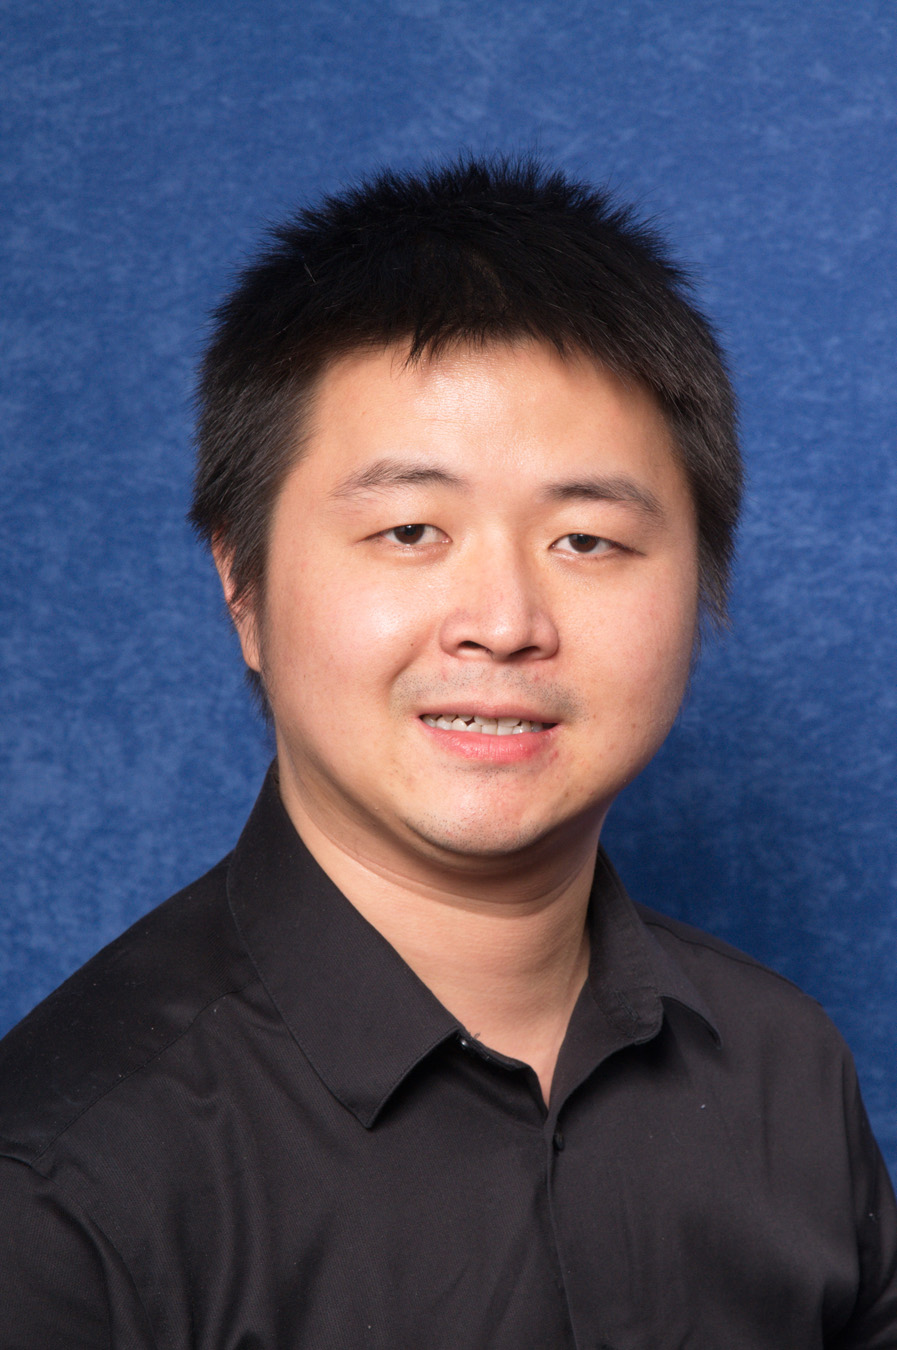
\includegraphics[width=1in,height=1.25in,clip,keepaspectratio]{bio/GuoJun_Qi.jpg}}]{Guo-Jun Qi}
Guo-Jun Qi (M14-SM18) is the Chief Scientist leading and overseeing an international R\&D team for multiple artificial intelligent services on the Huawei Cloud since August 2018. He was a faculty member in the Department of Computer Science and the director of MAchine Perception and LEarning (MAPLE) Lab at the University of Central Florida since August 2014. Prior to that, he was also a Research Staff Member at IBM T.J. Watson Research Center, Yorktown Heights, NY.
His research interests include machine learning and knowledge discovery from multi-modal data sources to build smart and reliable information and decision-making systems.
Dr. Qi has published more than 100 papers in a broad range of venues in pattern recognition, machine learning and computer vision.
He also has served or will serve as a general co-chair for ICME 2021, technical program co-chair for ACM Multimedia 2020, ICIMCS 2018 and MMM 2016, as well as an area chair (senior program committee member) for multiple academic conferences. Dr. Qi is an associate editor for IEEE Transactions on Circuits and Systems for Video Technology (T-CSVT), IEEE Transactions on Multimedia (T-MM), IEEE Transactions on Image Processing (T-IP), Pattern Recognition (PR), and ACM Transactions on Knowledge Discovery from Data (T-KDD).
\end{IEEEbiography}



\vspace{-12mm}
\begin{IEEEbiography}[{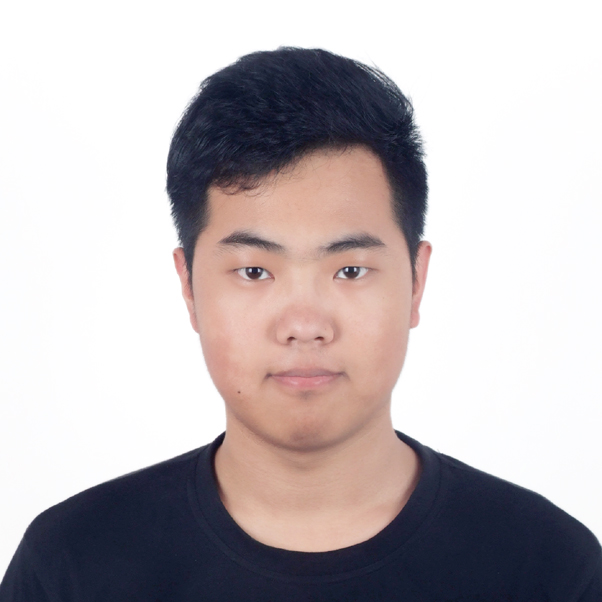
\includegraphics[width=1in,height=1.25in,clip,keepaspectratio]{bio/Liheng_Zhang.jpg}}]{Liheng Zhang}
Liheng Zhang received the B. S. degree in School of Electronic Information and Communications in Huazhong University of Science and Technology, in 2015. He is currently pursuing the PhD degree with the Department of Computer Science, University of Central Florida. His research interests include deep learning, machine learning and computer vision.
\end{IEEEbiography}

\vspace{-12mm}
\begin{IEEEbiography}[{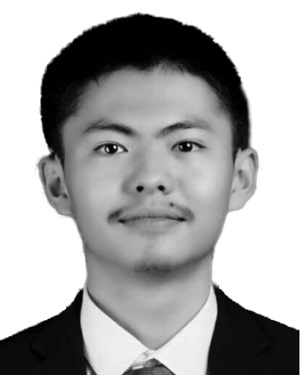
\includegraphics[width=1in,height=1.25in,clip,keepaspectratio]{bio/Xiao.jpg}}]{Xiao Wang}
Xiao Wang received the B.S. degree in Department of Computer Science in Xi'an Jiaotong University, in 2018. He is currently pursuing the PhD degree with the Department of Computer Science, Purdue University.  His research interests include deep learning, computer vision, bioinformatics and intelligent systems.
\end{IEEEbiography}
% You can push biographies down or up by placing
% a \vfill before or after them. The appropriate
% use of \vfill depends on what kind of text is
% on the last page and whether or not the columns
% are being equalized.

%\vfill

% Can be used to pull up biographies so that the bottom of the last one
% is flush with the other column.
%\enlargethispage{-5in}



% that's all folks
\end{document}


